%% =====================================================================
%% FedRouteAI B.Tech Major Project Report -- v2_citations
%% Auto-generated from "FEDROUTEAI DOC Final v1.00.docx".
%% Compiles on Overleaf with pdfLaTeX. Edit main.tex freely.
%% =====================================================================
\documentclass[12pt,a4paper,oneside]{report}

\usepackage[T1]{fontenc}
\usepackage[utf8]{inputenc}
\usepackage{newtxtext,newtxmath}   % Times New Roman look
\usepackage[a4paper,left=3.25cm,right=2.5cm,top=2.5cm,bottom=2.5cm]{geometry}
\usepackage{graphicx}
\graphicspath{{figures/}}
\usepackage{float}
\usepackage{array}
\usepackage{tabularx}
\usepackage{booktabs}
\usepackage{ragged2e}
\usepackage{setspace}
\usepackage{enumitem}
\usepackage[font=small,labelfont=bf,justification=centering,labelsep=colon]{caption}
\usepackage{titlesec}
\usepackage{fancyhdr}
\usepackage[colorlinks=true,linkcolor=black,citecolor=blue,urlcolor=blue,linktoc=all]{hyperref}
\usepackage{cleveref}

% ---- wrapping table column ----
\newcolumntype{L}{>{\RaggedRight\arraybackslash}X}

% ---- chapter / section styling ----
\titleformat{\chapter}[display]
  {\centering\normalfont\bfseries}
  {\Large CHAPTER-\thechapter}{1ex}{\LARGE}
\titlespacing*{\chapter}{0pt}{6pt}{26pt}
\titleformat{\section}{\normalfont\large\bfseries}{\thesection}{1em}{}
\titleformat{\subsection}{\normalfont\normalsize\bfseries}{\thesubsection}{1em}{}

% ---- footer: centered page number ----
\pagestyle{fancy}
\fancyhf{}
\fancyfoot[C]{\thepage}
\renewcommand{\headrulewidth}{0pt}
\fancypagestyle{plain}{\fancyhf{}\fancyfoot[C]{\thepage}\renewcommand{\headrulewidth}{0pt}}

\setlength{\parindent}{0.3in}
\onehalfspacing
\setlength{\parskip}{0.5em}

% ---- helper for centered institute block ----
\newcommand{\instituteblock}[1]{%
  \begin{center}
\includegraphics[width=3cm]{logo_bvrit.png}\\[4pt]
  {\Large\bfseries #1}\\[2pt]
  {\small Vishnupur, Narsapur, Medak, Telangana, India 502313}\end{center}}

\begin{document}
\pagenumbering{roman}


\thispagestyle{empty}
\begin{center}
{\large\bfseries A Major Project Phase-1 Report}\\[6pt]
{\large\bfseries On}\\[10pt]
{\large\bfseries FEDROUTEAI: ADAPTIVE FEDERATED LEARNING FOR RESILIENT EDGE-BASED TRAFFIC ANOMALY DETECTION}\\[14pt]
{In partial fulfillment of the requirements for the award of the degree}\\[4pt]
{\itshape Of}\\[6pt]
{\large\bfseries BACHELOR OF TECHNOLOGY}\\[4pt]
{\itshape In}\\[6pt]
{\large\bfseries Computer Science and Engineering (Data Science)}\\[16pt]
{Submitted by,}\\[8pt]
{\large MOGULOJU ABHIRAM (23211A6774)}\\[2pt]
{\large RAJULAPUDI ROHITH (23211A67A0)}\\[2pt]
\vspace{10pt}{Under the Guidance of}\\[4pt]
{\large\bfseries Mrs. S. Jyothsna}\\[2pt]
{Assistant Professor, Computer Science and Engineering (Data Science)}\\[14pt]

\includegraphics[width=3.2cm]{logo_bvrit.png}\\[10pt]
{\large\bfseries B V RAJU INSTITUTE OF TECHNOLOGY}\\[2pt]
{\small (An UGC Autonomous Institution, Approved by AICTE, New Delhi \& Affiliated to JNTUH, Hyderabad) Vishnupur, Narsapur, Medak, Telangana, India 502313}\\[10pt]
{\bfseries 2026 -- 2027}
\end{center}
\clearpage

\thispagestyle{empty}
\instituteblock{B V RAJU INSTITUTE OF TECHNOLOGY}
\vspace{6pt}\begin{center}{\Large\bfseries BONAFIDE CERTIFICATE}\end{center}\vspace{6pt}
\begin{justify}This is to certify that this major project work entitled ``FEDROUTEAI: ADAPTIVE FEDERATED LEARNING FOR RESILIENT EDGE-BASED TRAFFIC ANOMALY DETECTION'', submitted by MOGULOJU ABHIRAM (23211A6774), RAJULAPUDI ROHITH (23211A67A0) to B V Raju Institute of Technology affiliated to JNTUH, Hyderabad in partial fulfillment for the award of Bachelor of Technology in Computer Science and Engineering (Data Science) is a bonafide record of project work carried out under our supervision during the academic year 2026 -- 2027 and that this work has not been submitted elsewhere for a degree.\end{justify}
\vspace{28pt}
\noindent\textbf{SIGNATURE}\hfill\textbf{SIGNATURE}\\[2pt]
Mrs. S. Jyothsna\hfill Dr. R.V. Ramana Chary\\[1pt]
Supervisor\hfill Head of the Department\\[1pt]
Assistant Professor, CSD\hfill Professor, CSD
\vspace{34pt}
\noindent\textbf{Submitted for Major Project Phase-1 viva-voce examination held on}\\[26pt]
\noindent\textbf{INTERNAL EXAMINER}\hfill\textbf{EXTERNAL EXAMINER}

\clearpage
\instituteblock{B V RAJU INSTITUTE OF TECHNOLOGY}
\vspace{6pt}\begin{center}{\large\bfseries DECLARATION}\end{center}\vspace{6pt}
\begin{justify}We hereby declare that the project titled ``FEDROUTEAI: ADAPTIVE FEDERATED LEARNING FOR RESILIENT EDGE-BASED TRAFFIC ANOMALY DETECTION'', submitted to B V RAJU INSTITUTE OF TECHNOLOGY (Autonomous) and affiliated with JNTUH, Hyderabad, in partial fulfillment of the requirements for the award of a Bachelor of Technology in Computer Science and Engineering (Data Science), represents our ideas in our own words. Wherever others' ideas or words have been included, we have adequately cited and referenced the original sources. We also declare that we have adhered to all principles of academic honesty and integrity, and We have not misrepresented, fabricated, or falsified any idea, data, fact, or source in our submission. We understand that any violation of the above will be a cause for disciplinary action by the Institute. It is further declared that the project report or any part thereof has not been previously submitted to any University or Institute for the award of degree.\end{justify}
\vspace{30pt}\begin{flushright}\textbf{Signature(s)}\end{flushright}\vspace{6pt}
\noindent MOGULOJU ABHIRAM\hfill 23211A6774\\[2pt]
\noindent RAJULAPUDI ROHITH\hfill 23211A67A0\\[2pt]
\vspace{10pt}\noindent Place:\hspace{4cm}Date:

\clearpage
\instituteblock{B V RAJU INSTITUTE OF TECHNOLOGY}
\vspace{6pt}\begin{center}{\large\bfseries ACKNOWLEDGEMENT}\end{center}\vspace{6pt}
\begin{justify}We would like to express our sincere gratitude to the Management of BVRIT Narsapur, Dr. K. Lakshmi Prasad, Director and Dr. Sanjay Dubey, Principal for providing excellent infrastructure, necessary facilities, and a conducive academic environment for carrying out this Major Project Phase-1 successfully.\end{justify}\vspace{4pt}
\begin{justify}Our sincere thanks and gratitude to Dr. R.V. Ramana Chary, Professor \& Head of the Department of CSD for all the timely support and valuable suggestions during the period of Major Project Phase-1.\end{justify}\vspace{4pt}
\begin{justify}We are thankful to our Project Coordinator Dr Ch. Vengaiah, Assistant Professor, Department of CSD for his cooperation during the Major Project Phase-1.\end{justify}\vspace{4pt}
\begin{justify}We are greatly thankful and indebted to our internal guide, Mrs.S.Jyothsna, Assistant Professor, Department of CSD for her constant guidance, encouragement and moral support throughout the Major Project Phase-1.\end{justify}\vspace{4pt}
\begin{justify}Finally, we would also like to thank all the faculty and staff of the CSD Department who helped us directly or indirectly, parents and friends for their cooperation in completing Major Project Phase-1.\end{justify}\vspace{4pt}
\vspace{16pt}\begin{flushright}
MOGULOJU ABHIRAM\quad 23211A6774\\[2pt]
RAJULAPUDI ROHITH\quad 23211A67A0\\[2pt]
\end{flushright}

\clearpage
\begin{center}{\Large\bfseries ABSTRACT}\end{center}\vspace{8pt}
\begin{justify}FedRouteAI is a traffic intelligence system for detecting temporary road events from GPS-derived traffic behavior and supporting route inspection. The system combines geographically grounded synthetic traffic data, OpenStreetMap road geometry, PostGIS persistence, historical traffic memory, causal feature construction, federated learning, a frozen Geo V2 multilayer perceptron, and a React-Leaflet live map. Eight regional clients train locally and contribute model updates through FedAvg-style aggregation with adaptive weighting. Raw training or live traffic records are not required to be centralized for model inference. The current Geo V2 runtime uses an ordered 23-feature contract containing current traffic state, temporal encodings, road metadata, historical baselines, baseline deviations, prior-window trends, low-speed persistence, and directed-neighbor information. The model is executed in a label-free manner: scenario labels and ground-truth metadata are excluded from inference features. Live telemetry is ingested, associated with road segments, aggregated, combined with history, passed through the frozen model, and persisted as prediction state for the map. The system also imports a Beeramguda/Ashok Nagar OSM network containing 2,968 canonical segments and 11,259 directed transitions. The project includes a five-hour controlled demonstration with 1,000 persistent vehicles and 150 simulated ten-minute ticks. It also provides a route-bound demonstration in which the user calculates a directed route of at least 1.5 km and selects Normal, Congestion, or Accident behavior. Such scenario behavior is explicitly treated as demonstration traffic and not as model ground truth. The completed implementation demonstrates an end-to-end academic prototype while retaining clear limitations in event-class recall, data realism, operational privacy controls, and traffic-aware routing.\end{justify}\vspace{8pt}
\noindent\textbf{Keywords:} Federated Learning, Traffic Anomaly Detection, Geo V2, GPS Telemetry, Historical Traffic Memory, OpenStreetMap, PostGIS, Multilayer Perceptron, Adaptive FedAvg, Directed Routing

\clearpage
\renewcommand{\contentsname}{INDEX}
\tableofcontents
\clearpage
\addcontentsline{toc}{chapter}{LIST OF TABLES}
\renewcommand{\listtablename}{LIST OF TABLES}
\listoftables
\clearpage
\addcontentsline{toc}{chapter}{LIST OF FIGURES}
\renewcommand{\listfigurename}{LIST OF FIGURES}
\listoffigures

\clearpage
\begin{center}{\Large\bfseries LIST OF ABBREVIATIONS}\end{center}\vspace{8pt}
\renewcommand{\arraystretch}{1.3}
\noindent\begin{tabularx}{\textwidth}{@{}p{3cm} L@{}}
\toprule \textbf{Abbreviation} & \textbf{Description} \\ \midrule
AI & Artificial Intelligence \\
API & Application Programming Interface \\
F1 & Harmonic mean of precision and recall \\
FedAvg & Federated Averaging \\
FL & Federated Learning \\
FPR & False Positive Rate \\
GIS & Geographic Information System \\
GPS & Global Positioning System \\
Km/h & Kilometers per hour \\
M & Meters \\
MLP & Multilayer Perceptron \\
OSM & OpenStreetMap \\
PostGIS & PostgreSQL spatial database extension \\
REST & Representational State Transfer \\
V1 / V2 & Version 1 / Geo V2 system contracts \\
\bottomrule\end{tabularx}

\clearpage

\pagenumbering{arabic}

\chapter{INTRODUCTION}

\section{Introduction}

FedRouteAI is an adaptive federated learning~\cite{mcmahan2017,kairouz2021,beutel2020} system designed for traffic anomaly detection~\cite{elmanaa2022,raiyn2014,gao2023} using distributed~\cite{wu2024} GPS telemetry and spatial road-network information. The system combines federated learning, historical traffic memory, Geo V2 feature construction, machine learning-based traffic-event~\cite{han2019} classification, spatial processing, and directed routing into a unified traffic-intelligence platform. The proposed system is designed to process GPS-derived vehicle telemetry, associate observations with road segments, aggregate traffic conditions, construct a fixed set of Geo V2 features, and perform traffic-event prediction using a trained Multilayer Perceptron~\cite{goodfellow2016,bishop2006,paszke2019} (MLP) model. The prediction results are persisted and made available through application programming interfaces (APIs) for visualization through a web-based map interface. A key aspect of FedRouteAI is its federated learning architecture. Instead of requiring all regional training data to be collected at a single central location, the system represents eight regional clients that perform local model training. The resulting model updates are aggregated to produce a global model. Adaptive FedAvg~\cite{yuan2024,lu2024}~\cite{mcmahan2017} is used to provide weighted aggregation based on the regional training process. The system also incorporates OpenStreetMap~\cite{osm}-based road-network information and PostgreSQL~\cite{postgis}/PostGIS for spatial storage and processing. This enables GPS observations to be associated with canonical directed road segments and allows traffic conditions and predictions to be represented spatially. The project is implemented as an integrated prototype consisting of data processing, machine learning, backend API, database, frontend visualization, and routing components. The system is intended primarily as a reproducible academic prototype~\cite{projsrc} rather than a production-scale city-wide traffic management system.\par

\section{Background}

Modern transportation systems generate large volumes of mobility data through GPS-enabled vehicles and devices. Such data can provide useful information about vehicle movement, traffic conditions, road usage, and abnormal traffic events. However, converting raw GPS observations into meaningful traffic information requires several processing stages, including road-segment association, traffic aggregation, historical feature construction, machine learning inference, and spatial visualization. Traditional centralized machine learning approaches generally require training data from different sources or regions to be collected and processed centrally. In traffic applications, this can create challenges related to data ownership, communication~\cite{zhou2019,wang2020,khan2020}, scalability, and the handling of geographically distributed data. Federated learning provides an alternative approach in which participating clients train a shared model using their local data and communicate model updates rather than directly sharing the complete local training datasets. FedRouteAI applies this concept to regional traffic-event classification by representing eight regional clients and aggregating their locally trained models. The machine learning component of the system uses a Geo V2 feature representation containing 23 ordered input features. These features combine traffic, spatial, temporal~\cite{yang2022}, and historical information required by the trained MLP model. Maintaining the exact feature order and preprocessing configuration is an important part of the system because the runtime feature representation must remain compatible with the trained model artifact. The spatial component of FedRouteAI uses OpenStreetMap road-network information together with PostGIS. GPS observations are associated with road segments, and the resulting traffic information can be displayed geographically. The system also provides directed shortest-path routing using Dijkstra~\cite{dijkstra1959}'s algorithm. The current routing implementation is distance-based and is maintained separately from the machine learning prediction pipeline. Through the integration of these components, FedRouteAI provides a complete pipeline from distributed telemetry processing to traffic-event prediction, persistence, visualization, and route computation.\par

\section{Need for the Proposed System}

Traffic conditions can change rapidly because of congestion, accidents, abnormal vehicle movement, and other road events. A traffic-intelligence system therefore needs to process distributed mobility observations and transform them into useful segment-level information. A major challenge is that traffic data may originate from different geographic regions or organizations. A centralized approach can require the transfer and consolidation of large amounts of local data. Federated learning provides a mechanism for training a shared model while keeping the regional training process decentralized. Another requirement is the reliable conversion of raw GPS observations into meaningful road-level information. Latitude and longitude values alone do not directly represent the traffic condition of a particular road segment. Road-network association and aggregation are therefore required before traffic features can be supplied to the machine learning model. The proposed system addresses these requirements by combining distributed regional training with a standardized Geo V2 feature representation and a spatial road-network layer. The use of a fixed 23-feature contract provides consistency between training and inference, while the PostGIS-based spatial layer provides a common representation of road segments and traffic observations. The system also separates model-based traffic prediction from controlled traffic demonstrations, preventing demonstration scenario selection from being treated as ground truth for the model. Thus, FedRouteAI provides an integrated traffic-intelligence prototype that combines distributed learning, GPS-based traffic processing, spatial information, machine learning prediction, visualization, and routing.\par

\section{Contributions}

The project makes three primary implementation-level contributions. End-to-End Engineering Pipeline: FedRouteAI integrates traffic ingestion, road-segment association, traffic aggregation, historical memory, feature construction, model inference, prediction persistence, map visualization, and route inspection into a single end-to-end pipeline. Geo V2 Feature Contract: The Geo V2 runtime uses an ordered 23-feature contract covering current traffic state, temporal encodings, road metadata, historical baselines, baseline deviations, prior-window trends, low-speed persistence, and directed-neighbor information. The inference process is label-free, with scenario labels and ground-truth metadata excluded from the model input. Demonstration Workflow: The system provides controlled demonstrations for traffic conditions such as Normal, Congestion, and Accident. These demonstrations are kept separate from model predictions so that controlled traffic behavior is not incorrectly presented as learned model output.\par

\section{Scope of the Project}

The scope of FedRouteAI covers the design and implementation of an end-to-end prototype for distributed traffic-event detection and visualization. The system includes GPS telemetry ingestion and processing, road-segment association, traffic aggregation, historical traffic memory, Geo V2 feature construction, and MLP-based traffic-event prediction. The machine learning model operates on the defined 23-feature input representation and produces predictions corresponding to the traffic-event classes supported by the trained model. The federated learning component represents eight regional clients and supports local model training followed by aggregation into a global model. Adaptive FedAvg is incorporated into the federated aggregation process. The spatial layer uses OpenStreetMap-derived road-network information and PostgreSQL/PostGIS for storage and spatial processing. The processed traffic information and model predictions are exposed through backend APIs and visualized using a web-based frontend and map interface. The project also includes directed shortest-path routing using Dijkstra's algorithm. The routing functionality operates on the directed road network and is currently distance-based. Traffic predictions are not presently used as dynamic route-cost inputs. The project is intended to demonstrate the integration and reproducibility of these components in an academic environment. It does not claim production-scale deployment, continuously collected real-world traffic-data coverage, or operational city-wide traffic-management capability.\par

\section{Limitations}

The current implementation has several limitations that define the boundaries of the project. First, the Geo V2 dataset used for experimentation is geographically grounded synthetic data rather than a continuously collected real-world traffic dataset. Consequently, the reported model performance should be interpreted as experimental evidence for the implemented pipeline rather than as a measurement of real-world operational accuracy. Second, the dataset contains class imbalance~\cite{lu2024}, which affects the performance of minority traffic-event classes. The model therefore does not provide uniformly strong performance across all event categories. Third, the current routing implementation uses directed shortest-path routing based on distance. Although the system provides traffic-event predictions and route visualization, the predictions do not currently modify the route cost during path computation. Fourth, federated learning reduces the requirement to centralize raw training data, but federated learning alone does not guarantee privacy~\cite{liu2020}. The current prototype does not implement formal differential privacy~\cite{dwork2014,abadi2016,wei2020}, secure aggregation~\cite{kairouz2021,shokri2015}, or a formally defined privacy budget. Finally, production-scale deployment characteristics such as large-scale distributed ingestion, cloud deployment, end-to-end throughput, and long-term operational reliability have not been fully evaluated. These limitations are intentional boundaries of the current academic prototype and provide clear directions for future development.\par

\section{Organization of the Report}

This report presents the design, implementation, evaluation, and limitations of the FedRouteAI system. Chapter 1 introduces the project, its background, motivation, scope, and limitations. Chapter 2 presents the literature survey covering the major technologies and research areas related to federated learning, traffic anomaly detection, GPS trajector~\cite{zheng2015,su2019,li2018}y processing, spatial traffic analysis, and intelligent transportation systems~\cite{zhang2025,chen2016}. It also identifies the research gap addressed by the proposed system. Chapter 3 describes the system requirements and feasibility, including functional and non-functional requirements, stakeholders, system roles, dataset and model requirements, and feasibility considerations. Chapter 4 presents the system design and architecture, including the federated learning architecture, Geo V2 feature representation, traffic-processing pipeline, spatial database architecture, backend and frontend components, and routing architecture. Chapter 5 describes the implementation of the proposed system, including telemetry processing, feature construction, federated training, model inference, persistence, APIs, visualization, routing, and controlled demonstrations. Chapter 6 presents the testing and validation activities performed on the backend, frontend, machine learning pipeline, routing components, and overall system. The experimental results and model evaluation are also discussed. Chapter 7 discusses deployment, security, privacy considerations, performance measurements, and the practical limitations of the current implementation. Chapter 8 concludes the report and presents future enhancements that can extend the current prototype toward real-world datasets, traffic-aware routing, stronger privacy mechanisms, larger-scale federated learning, and production deployment.\par

\chapter{LITERATURE SURVEY}

\section{Federated Learning}

Federated learning~\cite{mcmahan2017,kairouz2021,beutel2020} is a distributed~\cite{wu2024} machine learning approach in which multiple participating clients train a shared model using their local data without directly transferring the complete local datasets to a central server. Instead of collecting all training data at one location, each client performs local training and communicates model updates for aggregation. Federated Averaging~\cite{mcmahan2017} (FedAvg) is one of the commonly used approaches for federated model aggregation. In FedAvg, locally trained model~\cite{goodfellow2016,bishop2006,paszke2019} parameters are combined to produce an updated global model. This approach provides a practical framework for collaborative model training when training data are distributed across different clients. Federated learning is particularly relevant to traffic-intelligence applications because mobility data can originate from different geographic regions, organizations, or data providers. Keeping the regional training process decentralized can reduce the requirement to centralize raw training data. FedRouteAI applies federated learning through eight regional clients. Each regional client participates in local model training, after which the local model updates are aggregated to obtain a global model. The system also incorporates Adaptive FedAvg~\cite{yuan2024,lu2024} to provide adaptive weighting during the aggregation process. However, federated learning should not be considered a complete privacy~\cite{liu2020} solution by itself. Model updates may still contain information that requires protection, and additional mechanisms such as differential privacy~\cite{dwork2014,abadi2016,wei2020} or secure aggregation~\cite{kairouz2021,shokri2015} may be required in a production environment. Such formal privacy mechanisms are outside the current scope of the prototype.\par

\section{Traffic Anomaly Detection}

Traffic anomaly detection~\cite{elmanaa2022,raiyn2014,gao2023} aims to identify traffic conditions or events that differ from normal road behavior, including congestion, accidents, and other traffic-related incident~\cite{han2019}s. GPS telemetry is useful for detecting these conditions because vehicle movement provides spatial and temporal~\cite{yang2022} information about road usage. However, raw GPS coordinates alone are insufficient for reliable road-level analysis, so observations must be associated with road segments and aggregated into meaningful traffic states. Machine learning techniques can classify traffic conditions using traffic, spatial, temporal, and historical features. FedRouteAI uses an MLP-based classification model for traffic-event prediction, operating on a fixed Geo V2 representation containing 23 ordered input features derived from processed traffic observations and associated information. The system separates model inputs from demonstration information, ensuring that controlled scenarios such as Normal, Congestion, and Accident are not directly supplied as prediction labels. This separation allows the demonstration mechanism and machine learning inference process to operate independently.\par

\section{GPS Trajectory and Spatial Processing}

GPS trajector~\cite{zheng2015,su2019,li2018}y data consist of sequences of geographic observations that can be used to study vehicle movement and road usage. Effective traffic analysis requires these observations to be connected to the underlying road network. Map matching or road-segment association is therefore an important stage in GPS-based traffic processing. It allows individual observations to be related to canonical road segments and enables traffic information to be aggregated at the road level. FedRouteAI uses OpenStreetMap~\cite{osm}-derived road-network information and PostgreSQL~\cite{postgis}/PostGIS for spatial storage and processing. GPS observations are associated with directed road segments, allowing the system to maintain a consistent spatial representation of the traffic network. Historical traffic information is also incorporated into the feature-construction process. Current traffic observations can therefore be considered together with previously stored traffic states when constructing the Geo V2 representation. The use of a canonical directed road network is important because road segments can have different directions of travel. Maintaining direction explicitly supports both traffic representation and the routing functionality provided by the system.\par

\section{Intelligent Transportation Systems}

Intelligent Transportation Systems~\cite{zhang2025,chen2016} (ITS) use sensing, communication~\cite{zhou2019,wang2020,khan2020}, computing, and data-analysis technologies to improve the monitoring and management of transportation networks. Modern ITS applications increasingly make use of GPS data, connected vehicles, machine learning, spatial databases, and web-based visualization. Traffic monitoring systems can provide information about road conditions and abnormal events, while predictive systems can use historical and current observations to estimate traffic states. Spatial visualization allows this information to be presented in a form that is easier to interpret and use. The integration of machine learning with distributed data processing provides an opportunity to develop traffic-intelligence systems that can operate across multiple geographic or organizational regions. Federated learning is particularly relevant in this context because it supports collaborative model training without requiring all local training data to be placed in a single repository. FedRouteAI combines these concepts into an integrated prototype. GPS-derived traffic observations are processed using a spatial road network, transformed into a standardized feature representation, evaluated using an MLP traffic-event classifier, and exposed through backend APIs for visualization. The system also provides directed shortest-path routing as a separate functionality.\par

\section{Research Gap}

Existing work in traffic intelligence generally focuses on individual aspects of the overall problem, such as traffic prediction, anomaly detection, trajectory analysis, federated learning, spatial processing, or route computation. These approaches demonstrate the usefulness of individual techniques, but an integrated system must also address the interfaces between these components. A practical traffic-intelligence pipeline requires consistent road-segment representation, reliable feature construction, compatibility between training and inference, distributed model training, prediction persistence, visualization, and route computation. It is also important to distinguish model-generated predictions from controlled demonstrations and to clearly define the limitations of the underlying data. FedRouteAI addresses this integration gap by combining distributed regional training, a fixed 23-feature Geo V2 representation, MLP-based traffic-event classification, GPS-to-road-segment processing, historical traffic memory, PostGIS-based spatial storage, API-based prediction access, map visualization, and directed shortest-path routing within one reproducible prototype. The contribution of the proposed system is therefore primarily the integration and reproducible implementation of these components into a unified traffic-intelligence workflow. The project does not claim that the individual techniques, such as federated learning, MLP classification, PostGIS processing, or Dijkstra~\cite{dijkstra1959} routing, are newly invented. Instead, it demonstrates how these established techniques can be combined into a common system architecture for distributed traffic-event analysis. The current implementation also provides a clear foundation for future work involving real-world traffic datasets, improved minority~\cite{lu2024}-class detection, traffic-aware route costs, stronger privacy mechanisms, larger federated deployments, and production-scale processing.\par

Table~\ref{tab:2-1} summarizes the Related Approaches and FedRouteAI Position.\par

\begin{table}[htbp]
\centering
\caption{Related Approaches and FedRouteAI Position}
\label{tab:2-1}
\renewcommand{\arraystretch}{1.25}
\begin{tabularx}{\textwidth}{@{}L L L@{}}
\toprule
\textbf{Area} & \textbf{Typical focus} & \textbf{FedRouteAI implementation} \\
\midrule
Traffic analysis & Speed, flow, and occupancy patterns & Current segment aggregates with historical comparison \\
Anomaly detection & Deviation or event classification & Frozen MLP with normal-history context \\
Federated learning & Distributed local training & Eight regional MLP clients and parameter aggregation \\
Spatial modeling & Road geometry and neighboring roads & OSM/PostGIS canonical directed topology \\
Routing & Shortest or alternative path & Directed distance-based route inspection \\
Visualization & Map and operational dashboard & React and Leaflet live traffic map \\
\bottomrule
\end{tabularx}
\end{table}

\chapter{REQUIREMENT ANALYSIS AND FEASIBILITY STUDY}

\section{Stakeholders and Core Requirements}

FedRouteAI involves multiple stakeholders who interact with or benefit from different parts of the system. The primary stakeholders include system administrators, traffic-data or regional clients, machine learning and data-processing components, and end users who access traffic information through the web interface. Regional clients represent geographically distributed~\cite{wu2024} sources of traffic data and participate in the federated learning~\cite{mcmahan2017,kairouz2021,beutel2020} process. They perform local model training using their respective regional data and contribute model updates to the global aggregation process. System administrators are responsible for managing the application environment, database, model artifact~\cite{goodfellow2016,bishop2006,paszke2019}s, configuration, and overall operation of the system. They may also monitor the status of the different system components. End users interact with the web application to view the road network, traffic conditions, predicted traffic event~\cite{han2019}s, vehicle movement, and available routes. The user interface provides a visual representation of the information produced by the backend processing pipeline. The machine learning and data-processing components form the computational part of the system. They process telemetry, construct features, perform model inference, store results, and provide information through the backend API.\par

\section{Functional Requirements}

The functional requirements define the main operations that FedRouteAI is expected to perform.\par

\smallskip\noindent\textbf{FR-01:} GPS Telemetry Ingestion\par

The system shall accept GPS-based vehicle telemetry containing the information required for traffic processing, including geographic position and relevant movement information.\par

\smallskip\noindent\textbf{FR-02:} Road-Segment Association\par

The system shall associate GPS observations with the appropriate road segments in the underlying road network.\par

\smallskip\noindent\textbf{FR-03:} Traffic Aggregation\par

The system shall aggregate processed vehicle observations to obtain segment-level traffic information.\par

\smallskip\noindent\textbf{FR-04:} Historical Traffic Processing\par

The system shall maintain and use historical traffic information as part of the feature-construction process.\par

\smallskip\noindent\textbf{FR-05:} Geo V2 Feature Construction\par

The system shall construct the defined Geo V2 feature representation containing 23 ordered input features required by the trained machine learning model.\par

\smallskip\noindent\textbf{FR-06:} Traffic-Event Prediction\par

The system shall perform traffic-event classification using the trained MLP model and produce predictions for the supported traffic-event classes.\par

\smallskip\noindent\textbf{FR-07:} Federated Learning\par

The system shall support regional model training using eight federated clients and aggregate the resulting local model updates into a global model using the implemented federated aggregation process.\par

\smallskip\noindent\textbf{FR-08:} Visualization and Routing\par

The system shall provide API-accessible traffic information for visualization through the web interface and shall support directed shortest-path routing using the available road network. The system shall also maintain a separation between model inference and controlled traffic demonstrations so that demonstration scenario selection is not directly treated as model ground truth.\par

\section{Non-Functional Requirements}

The non-functional requirements describe the quality and operational characteristics expected from the system.\par

Reproducibility: The system should provide a consistent feature representation, model artifact, configuration, and execution procedure so that the implemented workflow can be reproduced.\par

Model Compatibility: The runtime feature vector must maintain the same ordering and preprocessing requirements as the model used during training.\par

Spatial Consistency: Traffic observations, predictions, and routes should use a consistent directed road-network representation.\par

Performance: The system should provide sufficiently responsive model inference and application-level processing for the intended academic prototype~\cite{projsrc} and demonstration environment.\par

Reliability: The backend, database, model inference, and frontend components should operate together without introducing invalid or inconsistent traffic information.\par

Maintainability: The system should maintain separation between data processing, machine learning, database, API, frontend, and routing responsibilities.\par

Usability: The web interface should provide an understandable representation of road conditions, predictions, vehicles, and routes.\par

\section{System Roles}

FedRouteAI uses different roles according to the responsibilities performed by each component or participant.\par

Regional Client: A regional client performs local training using its available regional data and contributes the resulting model update to the federated learning process.\par

Federated Aggregator: The aggregation component combines the local model updates from participating regional clients to produce the global model.\par

Backend System: The backend manages telemetry processing, feature construction, model inference, prediction persistence, API operations, and communication~\cite{zhou2019,wang2020,khan2020} with the spatial database.\par

Database: PostgreSQL~\cite{postgis}/PostGIS stores the spatial road network, traffic-related information, and persisted prediction information required by the application.\par

Frontend User: The frontend user accesses the web application to view traffic information, model predictions, vehicle movement, and routes.\par

\section{Dataset and Model Requirements}

The machine learning pipeline requires a consistent dataset and feature representation. The Geo V2 representation used by FedRouteAI contains 23 ordered input features. The feature order and preprocessing configuration must remain consistent between model training and runtime inference. The dataset used for experimentation is geographically grounded synthetic traffic data. It provides the observations required to develop and evaluate the traffic-event classification pipeline while maintaining a controlled experimental environment. The model is an MLP-based classifier trained for the supported traffic-event classes. The trained model artifact is used during runtime inference, and the feature-construction pipeline must produce an input representation compatible with the stored model. The dataset contains class imbalance~\cite{lu2024}, particularly among some traffic-event categories. Therefore, evaluation results should be interpreted with appropriate class-level and macro-averaged metrics rather than relying only on overall accuracy. The system also requires road-network information for spatial processing. OpenStreetMap~\cite{osm}-derived road-network data and PostGIS provide the spatial foundation for associating GPS observations with road segments and representing the directed road network.\par

\section{Feasibility Analysis}

\subsection*{Technical Feasibility}

The proposed system is technically feasible using the technologies selected for the implementation. Machine learning functionality can be implemented using Python-based tools, while PostgreSQL/PostGIS provides the required spatial storage and processing capabilities. FastAPI~\cite{fastapi} provides the backend API layer, and the React~\cite{react_leaflet}-based frontend supports web visualization. The federated learning workflow can be implemented using regional client simulations and a central aggregation process. The use of a fixed 23-feature representation also provides a clear interface between feature construction and model inference.\par

\subsection*{Operational Feasibility}

The system is designed to provide an integrated workflow that can be operated in an academic development environment. Users can access the web interface to view the road network, traffic information, predictions, and routing results. The modular separation between ingestion, processing, machine learning, persistence, API, frontend, and routing components supports development and testing of individual parts of the system.\par

\subsection*{Economic Feasibility}

The project uses open-source technologies and publicly available road-network information. This reduces software licensing requirements and makes the prototype suitable for development using commonly available computing resources. The current implementation is intended as an academic prototype and does not require the infrastructure associated with production-scale city-wide deployment.\par

\section{Ethical Considerations and Constraints}

Traffic and mobility information can contain sensitive movement patterns, so FedRouteAI uses decentralized training to reduce the need to centralize raw regional training data. However, federated learning alone does not provide complete privacy~\cite{liu2020} protection, as the current implementation does not include differential privacy~\cite{dwork2014,abadi2016,wei2020} or secure aggregation~\cite{kairouz2021,shokri2015}. The project also has limitations due to the use of synthetic data, which is useful for controlled experimentation but does not replace evaluation with continuously collected real-world traffic data. The current routing functionality provides directed shortest-path routing based on distance and does not use traffic-event predictions as dynamic route costs. Therefore, FedRouteAI is intended as a reproducible academic prototype demonstrating the integration of distributed learning, traffic processing, spatial information, machine learning, visualization, and routing rather than a production-ready traffic-management platform.\par

Table~\ref{tab:3-1} summarizes the Functional Requirements.\par

\begin{table}[htbp]
\centering
\caption{Functional Requirements}
\label{tab:3-1}
\renewcommand{\arraystretch}{1.25}
\begin{tabularx}{\textwidth}{@{}L L L@{}}
\toprule
\textbf{ID} & \textbf{Requirement} & \textbf{Verification} \\
\midrule
FR-01 & Ingest GPS or trusted live observations & API and integration tests \\
FR-02 & Associate observations with road segments & Map-matching and network tests \\
FR-03 & Construct historical and Geo V2 features & Feature-contract checks \\
FR-04 & Run frozen MLP inference & Artifact and prediction tests \\
FR-05 & Persist and serve prediction state & Live map API tests \\
FR-06 & Display roads, vehicles, events, and predictions & Frontend tests and build \\
FR-07 & Calculate directed shortest routes & Routing tests \\
FR-08 & Run route-bound demonstrations & Demo validation tests \\
\bottomrule
\end{tabularx}
\end{table}

Table~\ref{tab:3-2} summarizes the Requirement Traceability.\par

\begin{table}[htbp]
\centering
\caption{Requirement Traceability}
\label{tab:3-2}
\renewcommand{\arraystretch}{1.25}
\begin{tabularx}{\textwidth}{@{}L L@{}}
\toprule
\textbf{Requirement group} & \textbf{Primary implementation evidence} \\
\midrule
Data & Geo V2 manifest, feature builder, and dataset partitions \\
Model & Feature schema, model store, frozen artifact metadata \\
Network & Cached OSM JSON, network normalizer, PostGIS import \\
Runtime & Live ingestion, snapshot, prediction persistence \\
User interface & Traffic Map tests, route planner, scenario controls \\
Validation & Backend suite, frontend suite, build, compile, and smoke evidence \\
\bottomrule
\end{tabularx}
\end{table}

\chapter{SYSTEM DESIGN AND ARCHITECTURE}

\section{Overall System Architecture}

FedRouteAI is designed as an end-to-end~\cite{projsrc} traffic-intelligence system that connects distributed~\cite{wu2024} traffic-data processing, federated learning~\cite{mcmahan2017,kairouz2021,beutel2020}, machine learning inference, spatial storage, backend services, web visualization, and routing. The overall architecture consists of regional data-processing clients, a federated learning aggregation layer, the trained traffic-event~\cite{han2019} classification model, a spatial database, backend APIs, and a web-based frontend. The architecture separates the training workflow from the runtime inference and visualization workflow while maintaining a common feature and road-network representation. At the regional level, traffic data are processed locally by participating clients. Each client prepares the required training information and performs local model training. The resulting model updates are communicated to the federated aggregation process, where they are combined to produce the global model. During runtime, GPS telemetry is processed through a sequence of stages. Vehicle observations are associated with road segments and aggregated to obtain traffic information. Historical traffic information is then combined with current observations to construct the Geo V2 feature representation. The resulting feature vector is passed to the trained MLP~\cite{goodfellow2016,bishop2006,paszke2019} model for traffic-event prediction. The prediction results are persisted through the backend and made available through APIs. The frontend consumes this information and displays traffic conditions, predicted events, vehicle movement, and the road network on an interactive map. Routing is implemented as a separate component of the system. Origin and destination points are associated with the directed road network, after which Dijkstra~\cite{dijkstra1959}'s algorithm is used to determine a shortest path. The current routing implementation is distance-based and does not use the machine learning prediction as a dynamic route cost. The overall processing flow can therefore be represented as:\par

\begin{center}\ttfamily\small Telemetry  $\rightarrow$  Segment Association  $\rightarrow$  Traffic Aggregation  $\rightarrow$  Historical Traffic Processing  $\rightarrow$  Geo V2 Feature Construction  $\rightarrow$  MLP Inference  $\rightarrow$  Prediction Persistence  $\rightarrow$  API  $\rightarrow$  Map Visualization\end{center}

Routing operates alongside this workflow using the directed road network.\par

The Overall System Architecture of FedRouteAI is illustrated in Figure~\ref{fig:4-1}.\par

\begin{figure}[p]
\centering
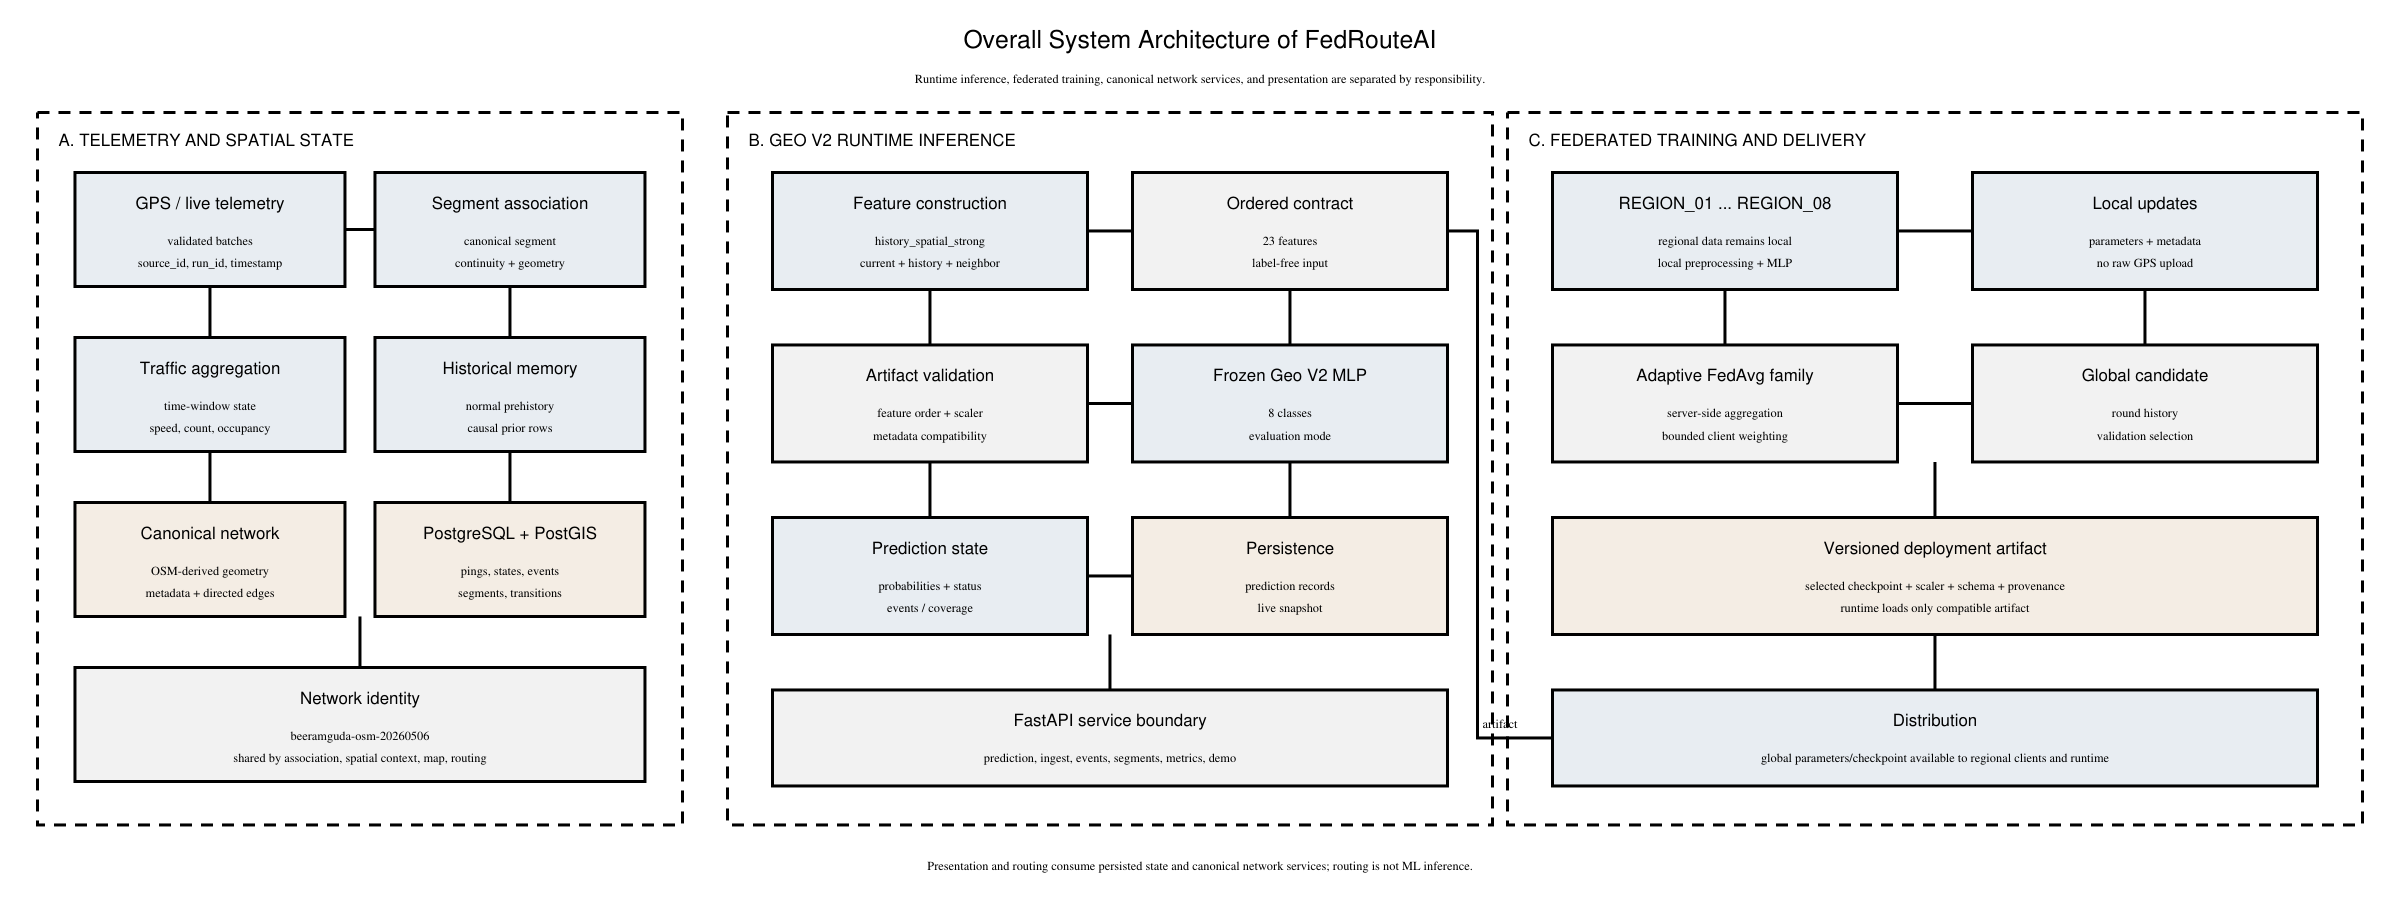
\includegraphics[width=0.9\textwidth,height=0.82\textheight,keepaspectratio]{fig_4_1.png}
\caption{Overall System Architecture of FedRouteAI}
\label{fig:4-1}
\end{figure}

\section{Federated Learning Architecture}

The federated learning architecture represents eight regional clients participating in collaborative model training. Each regional client maintains its local training data and performs local model training without requiring the complete raw training dataset to be transferred to a central location. After local training, the participating clients provide their model updates to the aggregation process. The aggregation mechanism combines the regional updates to obtain a global model. FedAvg~\cite{mcmahan2017} provides the basic federated aggregation approach, while Adaptive FedAvg~\cite{yuan2024,lu2024} is incorporated to provide adaptive weighting of regional contributions. The federated architecture separates the regional training process from the global model aggregation process. This allows the system to represent geographically distributed traffic-data sources while maintaining a common machine learning model.\par

The resulting global model is used as the trained model artifact for the prediction pipeline. The runtime system therefore does not need to repeat federated training for every prediction request. The federated architecture should not be interpreted as providing complete privacy~\cite{liu2020} protection. Raw training data remain decentralized within the intended workflow, but formal mechanisms such as differential privacy~\cite{dwork2014,abadi2016,wei2020} and secure aggregation~\cite{kairouz2021,shokri2015} are not implemented in the current prototype.\par

\section{Geo V2 Feature Design}

The Geo V2 feature representation provides the interface between traffic processing and the machine learning model. The model expects a fixed set of 23 ordered input features. Maintaining this feature contract is essential because a change in feature order, preprocessing, or representation can cause incompatibility between the training and runtime inference stages. The features are constructed from the processed traffic state together with spatial, temporal~\cite{yang2022}, and historical information available to the system. Current observations are combined with historical traffic information to provide the model with information about the recent state of a road segment. The Geo V2 representation is designed to provide a consistent input structure for the MLP classifier. The same feature ordering and preprocessing requirements used during training must be followed during runtime inference. The traffic-event label or controlled demonstration selection is not used as a direct model input. This maintains a separation between the information available to the model and the scenario used to demonstrate system behavior. The Geo V2 feature contract is therefore an important architectural boundary:\par

\begin{center}\ttfamily\small Traffic and spatial information  $\rightarrow$  23 ordered features  $\rightarrow$  preprocessing  $\rightarrow$  MLP model\end{center}

This boundary supports reproducibility and reduces the possibility of training-serving feature mismatch.\par

\section{Traffic Processing Pipeline}

The traffic processing pipeline converts raw GPS-derived observations into segment-level information suitable for machine learning inference. The first stage receives vehicle telemetry containing geographic and movement information. These observations are associated with the appropriate road segments in the underlying road network. After segment association, observations are aggregated to obtain road-level traffic information. Aggregation provides a more useful representation of traffic conditions than individual GPS observations because multiple vehicle observations can be considered together. Historical traffic information is maintained and retrieved as part of the feature-construction process. Current traffic observations and historical information are then used to construct the Geo V2 representation. The resulting 23-feature vector is passed to the trained MLP classifier. The model produces a traffic-event prediction, which is persisted and subsequently made available through the backend API. The complete pipeline maintains a separation between raw telemetry, processed traffic state, model features, model prediction, and visualization. This separation makes it possible to test individual stages and reduces the risk of information from later stages being incorrectly used during earlier processing.\par

\section{Database and Spatial Architecture}

PostgreSQL~\cite{postgis} with PostGIS provides the spatial storage layer of FedRouteAI. The database stores the road-network information and spatially related traffic and prediction information required by the application. OpenStreetMap~\cite{osm}-derived road-network information provides the underlying geographic representation. Road segments are represented as directed network elements so that the system can distinguish between different travel directions where required. GPS observations are associated with these canonical road segments. This allows traffic information to be represented consistently across the processing, prediction, visualization, and routing components. The spatial database also provides the persistence layer for information generated by the runtime pipeline. Backend services interact with the database to store and retrieve traffic-related information and model predictions. Using a common spatial representation ensures that the road displayed on the frontend corresponds to the road used during traffic processing and routing.\par

\section{Backend and Frontend Architecture}

The backend provides the application services required to connect the traffic-processing and machine-learning components with the web interface. FastAPI~\cite{fastapi} is used to expose API endpoints through which the frontend can retrieve traffic information, predictions, road-network information, and routing results. The backend follows a modular structure separating responsibilities such as API handling, application services, machine learning, data processing, and database access. This separation supports maintainability and allows individual components to be tested independently. The frontend is implemented using React~\cite{react_leaflet} and provides the user-facing interface for the system. It communicates with the backend through the defined APIs and presents traffic information using an interactive map interface. The frontend displays information such as the road network, vehicle movement, traffic conditions, predicted events, and route information. The map-based interface provides a visual representation of the spatial information produced by the backend. The frontend and backend therefore form a separate application layer above the data-processing and spatial-storage components:\par

\begin{center}\ttfamily\small Frontend  $\rightarrow$  API  $\rightarrow$  Backend Services  $\rightarrow$  Database / ML / Processing Components\end{center}

This architecture keeps presentation logic separate from the underlying traffic and machine-learning operations.\par

\section{Routing Architecture}

FedRouteAI provides directed shortest-path routing using the road network stored in the spatial database. The routing process accepts an origin and destination and identifies the corresponding locations in the directed road network. Dijkstra's algorithm is then used to compute a shortest path through the available directed road segments. The resulting path can be returned through the backend and displayed through the frontend map interface. The routing component is intentionally separated from the traffic-event prediction pipeline. The current implementation uses distance-based routing, meaning that the predicted traffic-event class does not automatically change the cost of a road segment during route computation. This separation provides a clear architectural boundary between traffic-event classification and route computation. A future traffic-aware routing implementation could use predicted traffic conditions as dynamic route costs, but such functionality is outside the current implementation. The resulting architecture therefore supports two related but distinct capabilities:\par

\begin{center}\ttfamily\small Traffic intelligence: \\ GPS telemetry  $\rightarrow$  traffic processing  $\rightarrow$  Geo V2 features  $\rightarrow$  MLP prediction\end{center}

\begin{center}\ttfamily\small Route computation: \\ Origin/Destination  $\rightarrow$  Directed Road Network  $\rightarrow$  Dijkstra  $\rightarrow$  Shortest Path\end{center}

Together, these components provide the foundation for the FedRouteAI traffic-intelligence prototype.\par

Table~\ref{tab:4-1} summarizes the Dataset and Runtime Data Separation.\par

\begin{table}[htbp]
\centering
\caption{Dataset and Runtime Data Separation}
\label{tab:4-1}
\renewcommand{\arraystretch}{1.25}
\begin{tabularx}{\textwidth}{@{}L L L@{}}
\toprule
\textbf{Data source} & \textbf{Purpose} & \textbf{Labels available?} \\
\midrule
ML training/evaluation data & Train, validate, and test the classifier & Yes for target construction/evaluation \\
OSM/PostGIS network & Geometry, road metadata, topology, and routing & No \\
Live GPS telemetry & Current runtime observations & No scenario labels in inference \\
Controlled demonstration telemetry & Repeatable route-bound behavior & Scenario truth kept outside features \\
Prediction persistence & Serve independent model outputs & Predicted class and confidence \\
\bottomrule
\end{tabularx}
\end{table}

The Federated Learning Architecture is illustrated in Figure~\ref{fig:4-2}.\par

\begin{figure}[p]
\centering
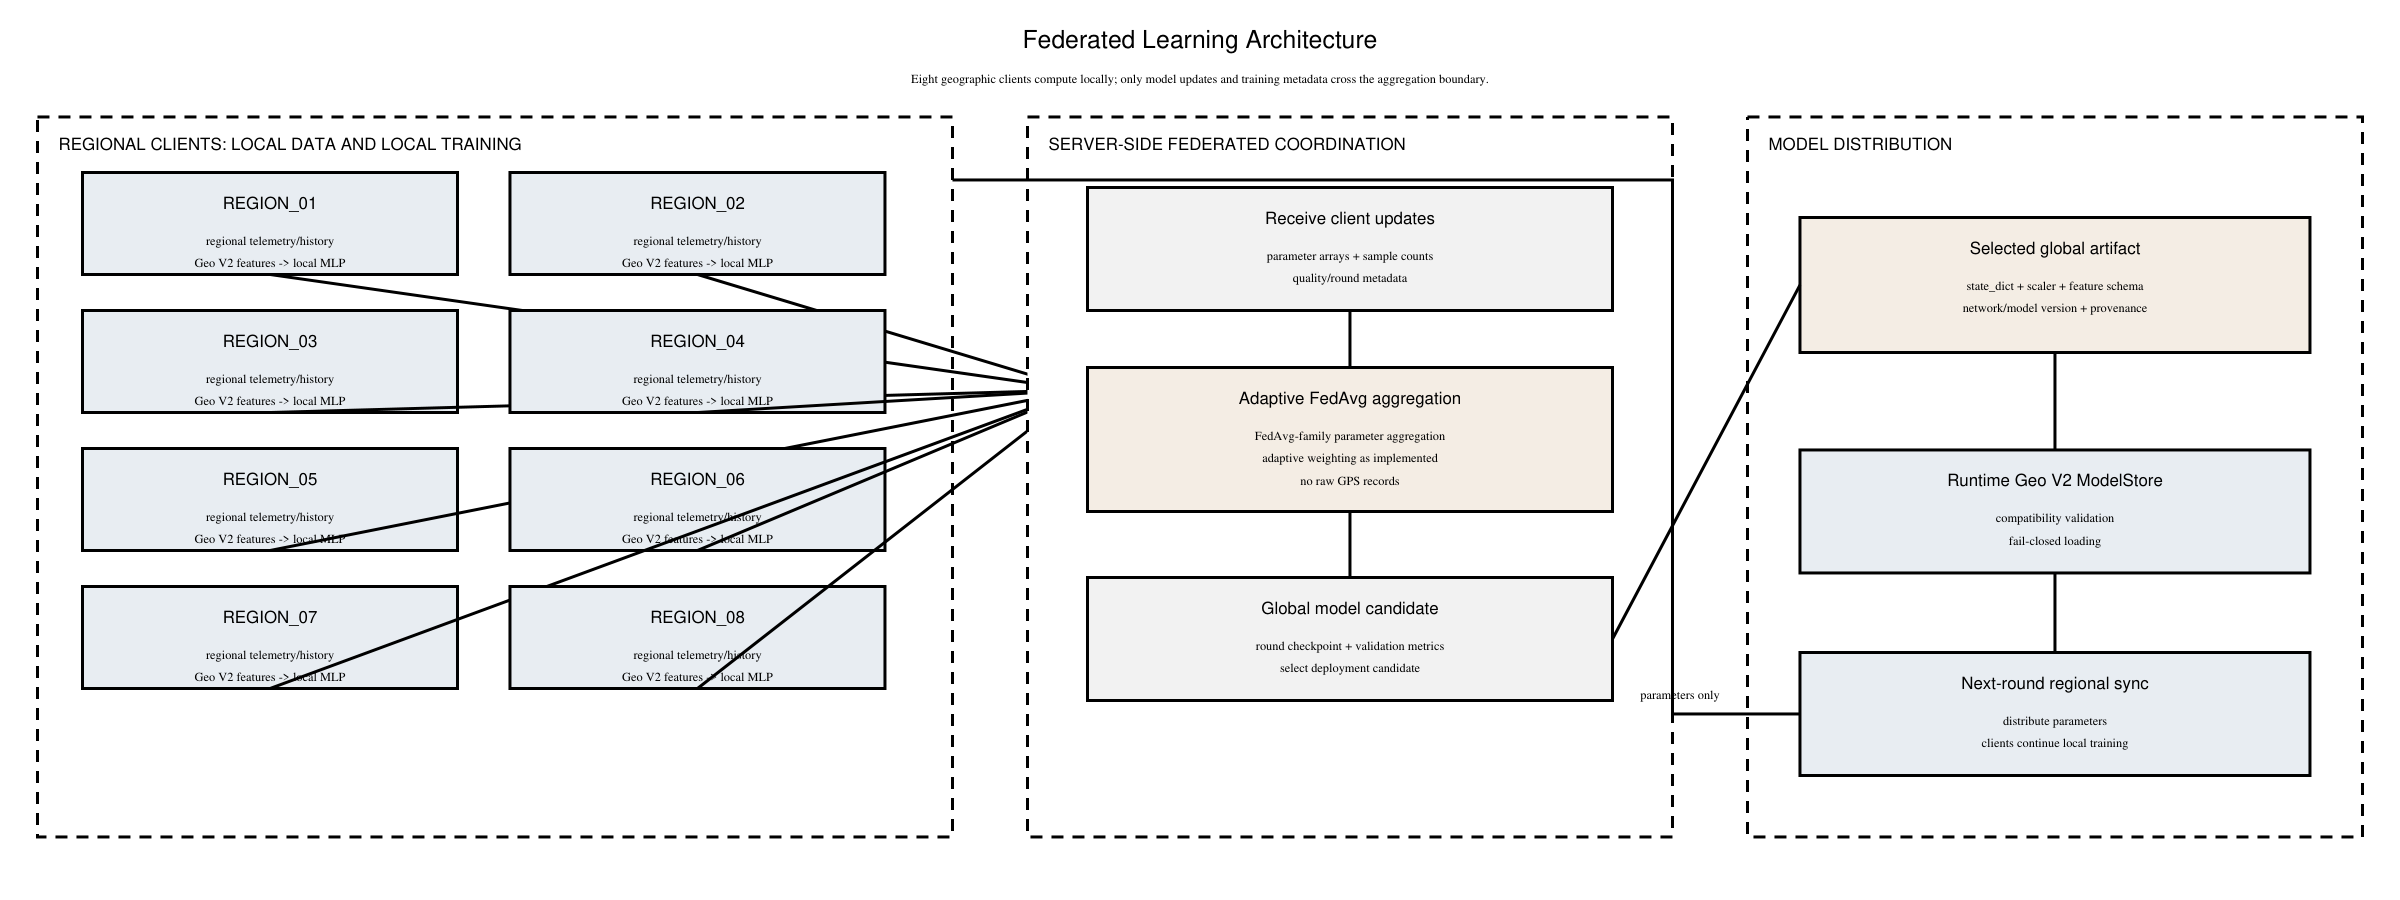
\includegraphics[width=0.9\textwidth,height=0.82\textheight,keepaspectratio]{fig_4_2.png}
\caption{Federated Learning Architecture}
\label{fig:4-2}
\end{figure}

The Regional Client and Server Interaction is illustrated in Figure~\ref{fig:4-3}.\par

\begin{figure}[p]
\centering
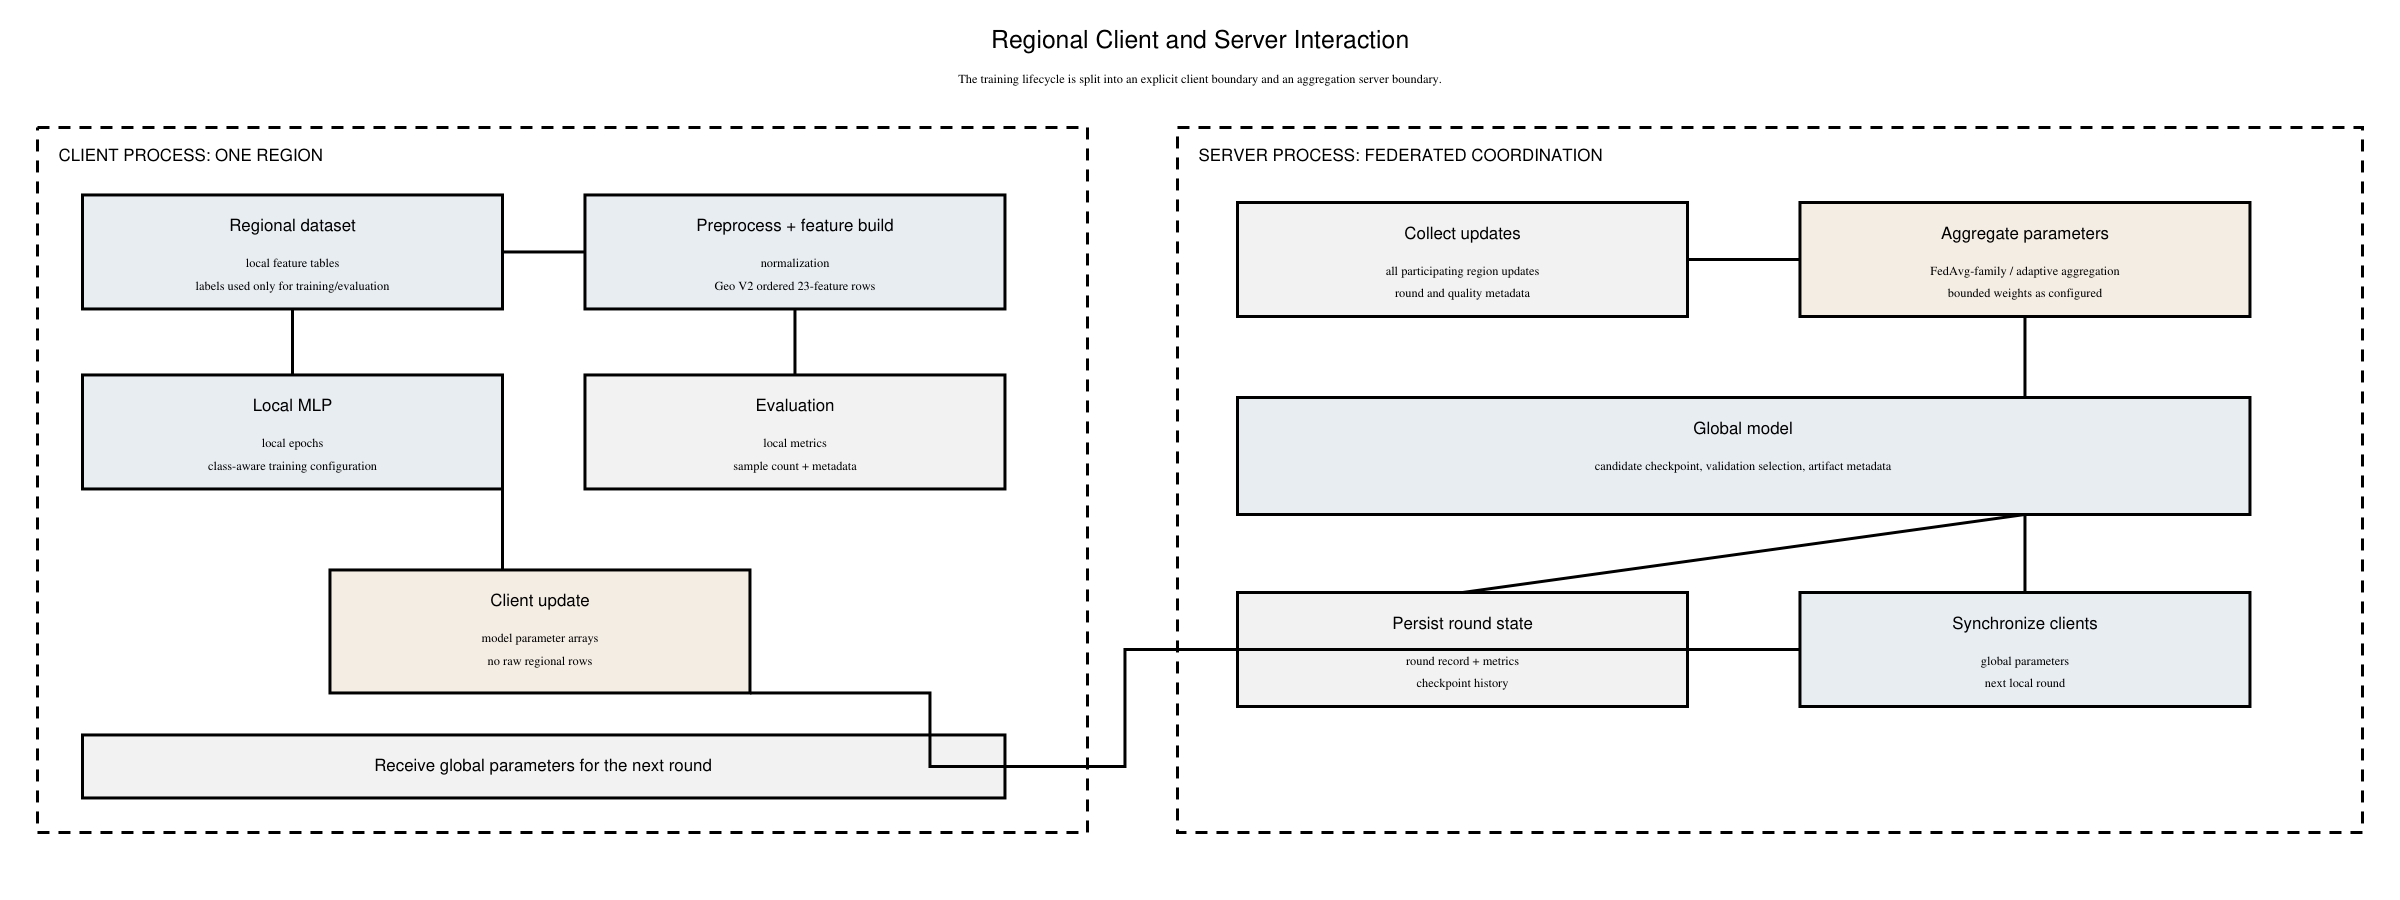
\includegraphics[width=0.9\textwidth,height=0.82\textheight,keepaspectratio]{fig_4_3.png}
\caption{Regional Client and Server Interaction}
\label{fig:4-3}
\end{figure}

The End-to-End Data Pipeline is illustrated in Figure~\ref{fig:4-4}.\par

\begin{figure}[p]
\centering
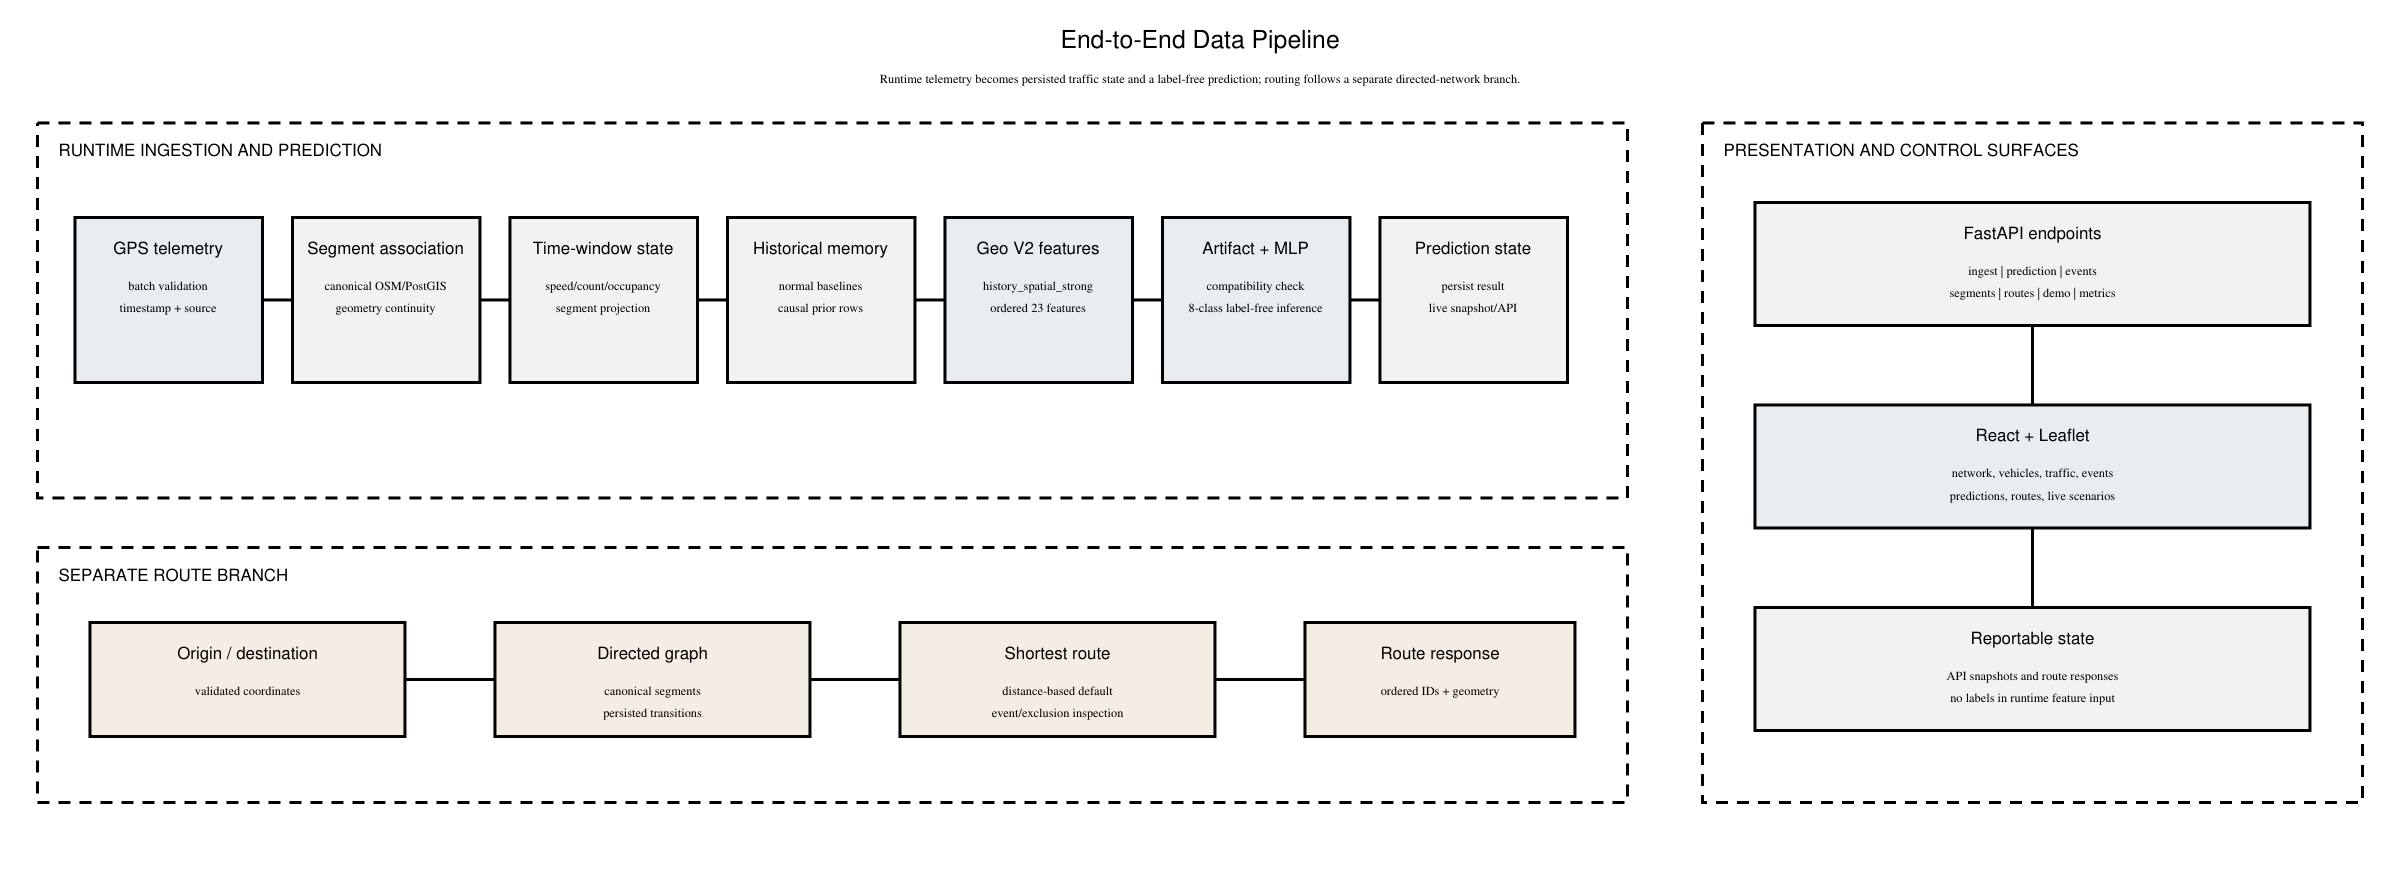
\includegraphics[width=0.9\textwidth,height=0.82\textheight,keepaspectratio]{fig_4_4.png}
\caption{End-to-End Data Pipeline}
\label{fig:4-4}
\end{figure}

The Geo V2 Feature Construction Pipeline is illustrated in Figure~\ref{fig:4-5}.\par

\begin{figure}[p]
\centering
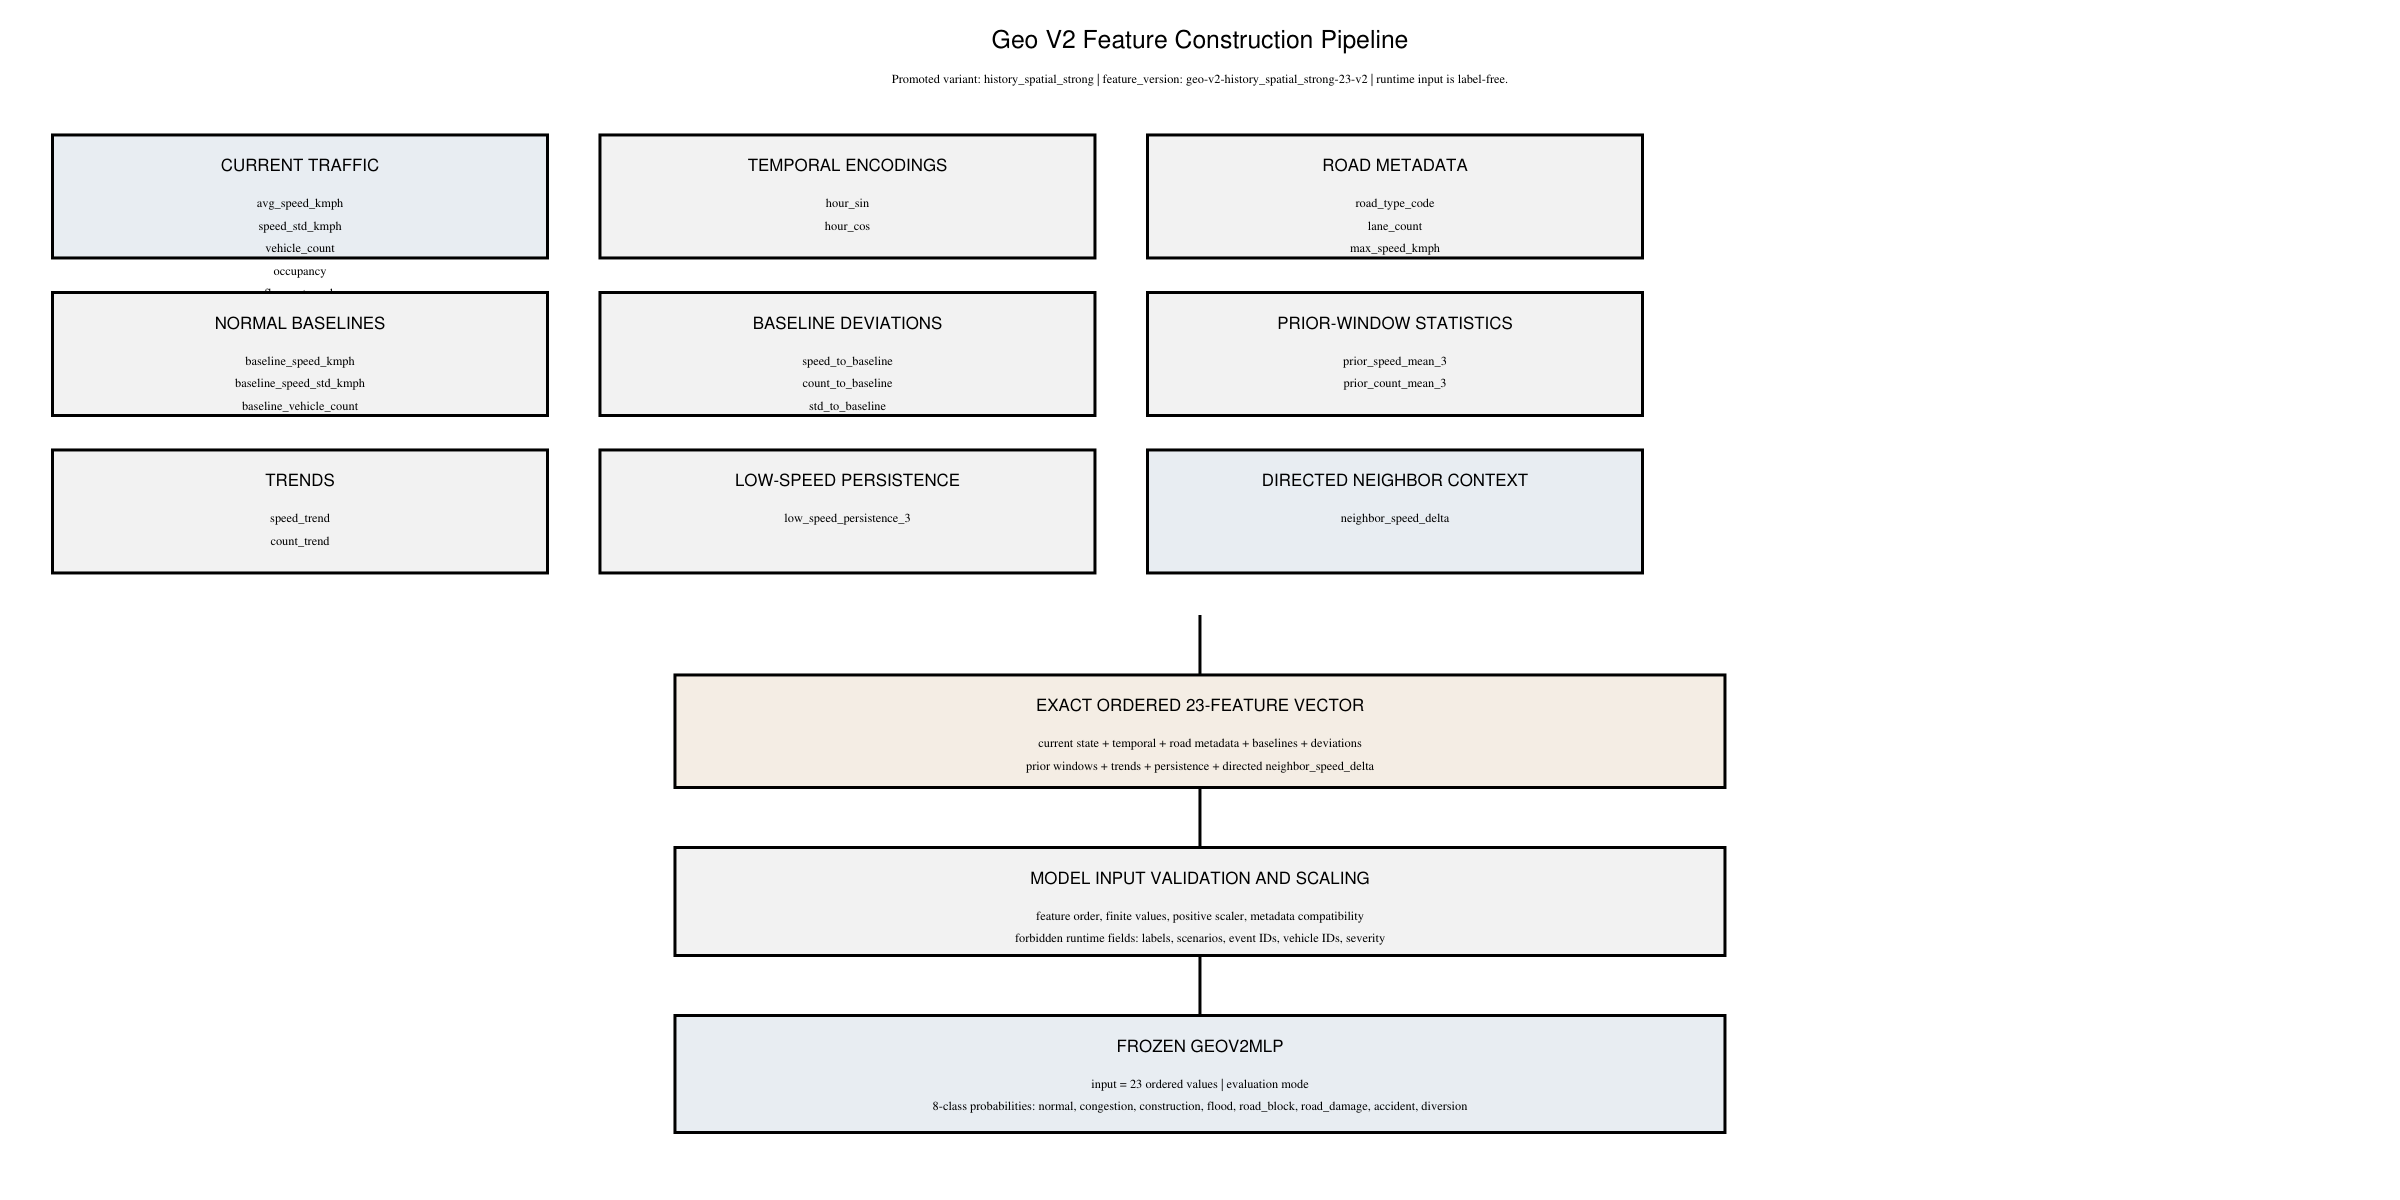
\includegraphics[width=0.9\textwidth,height=0.82\textheight,keepaspectratio]{fig_4_5.png}
\caption{Geo V2 Feature Construction Pipeline}
\label{fig:4-5}
\end{figure}

The Historical Traffic Memory and Causal Windows is illustrated in Figure~\ref{fig:4-6}.\par

\begin{figure}[p]
\centering
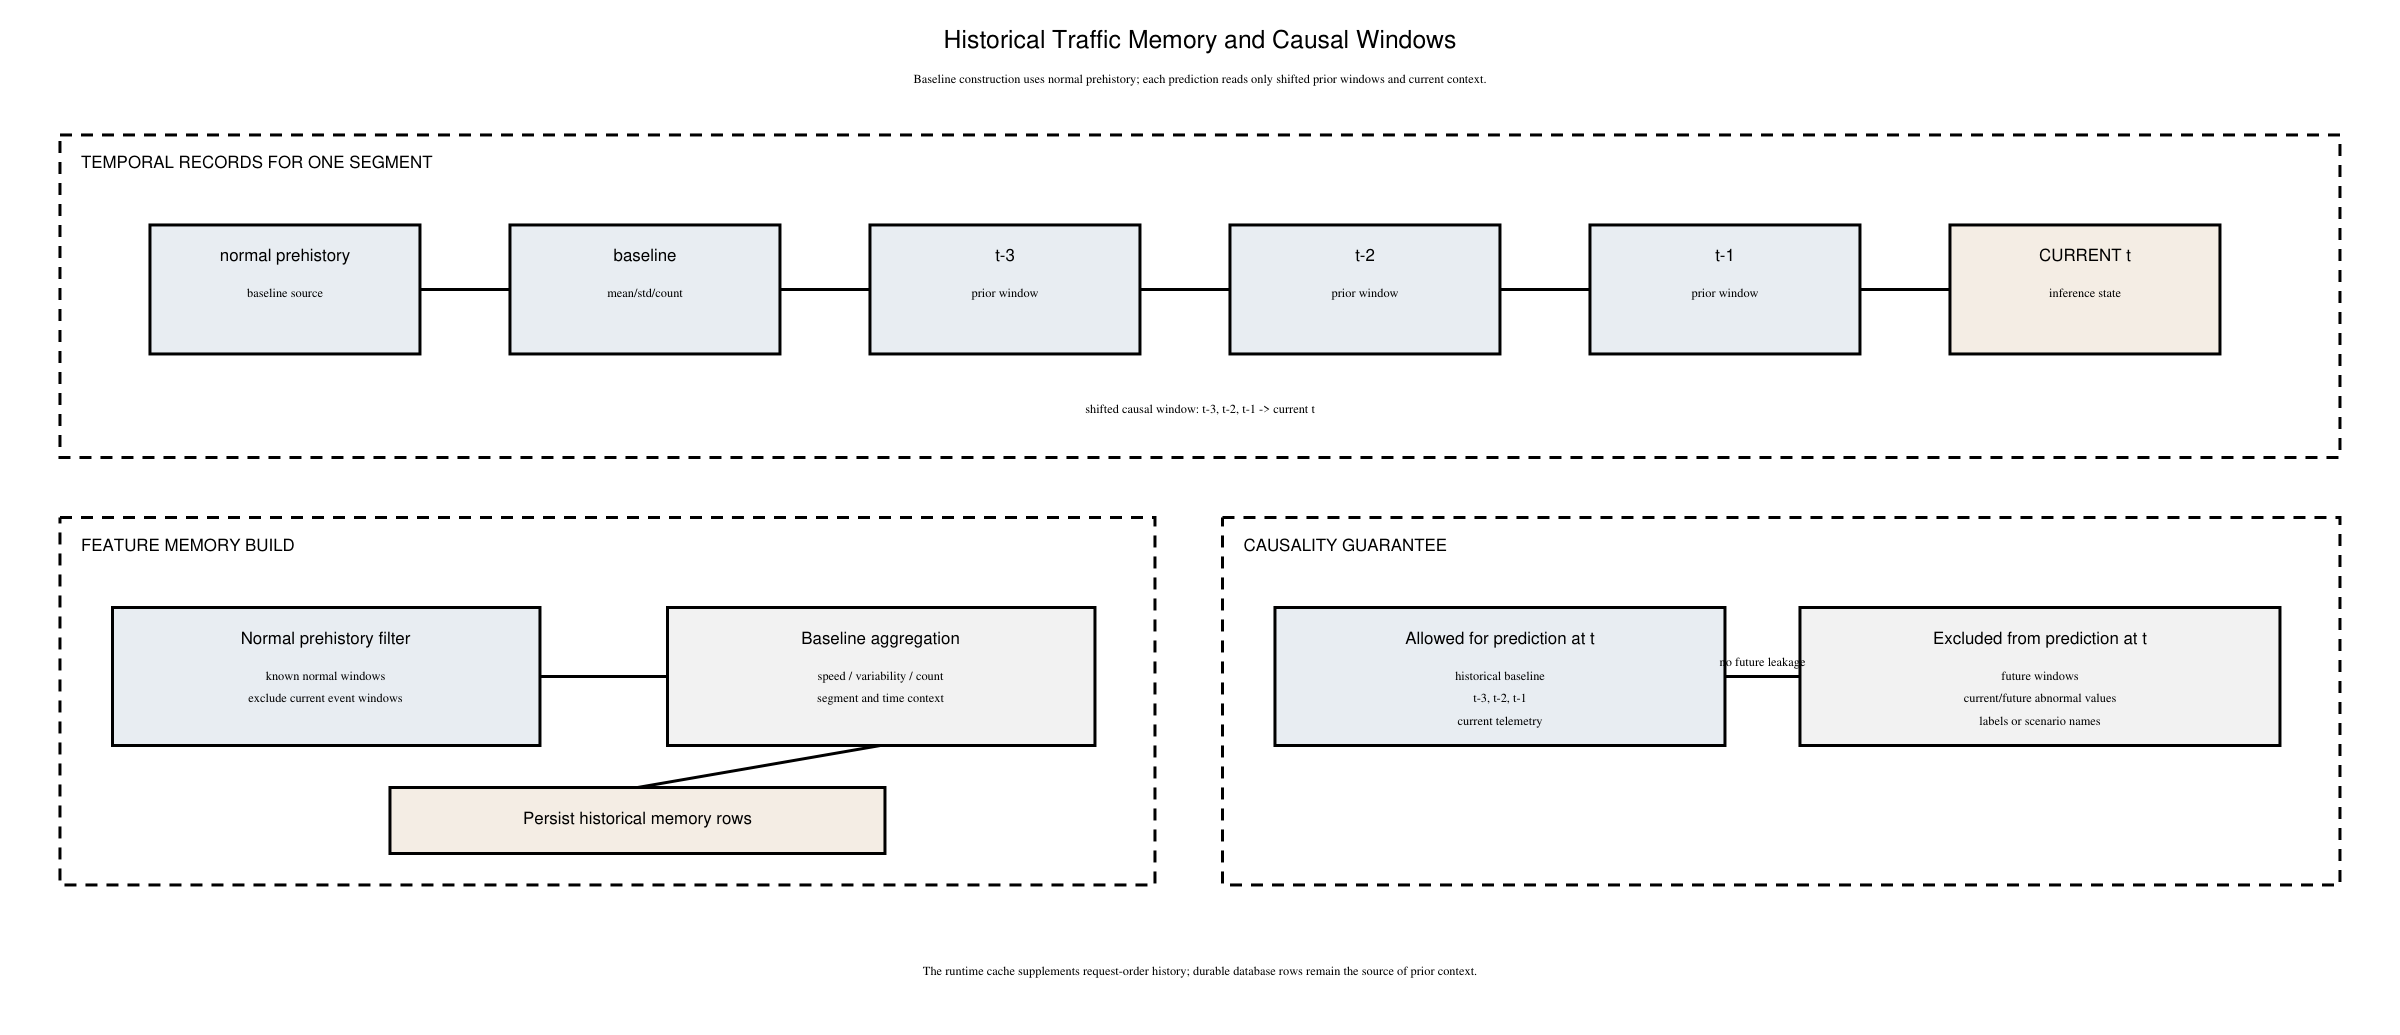
\includegraphics[width=0.9\textwidth,height=0.82\textheight,keepaspectratio]{fig_4_6.png}
\caption{Historical Traffic Memory and Causal Windows}
\label{fig:4-6}
\end{figure}

The OSM/PostGIS Network Import is illustrated in Figure~\ref{fig:4-7}.\par

\begin{figure}[p]
\centering
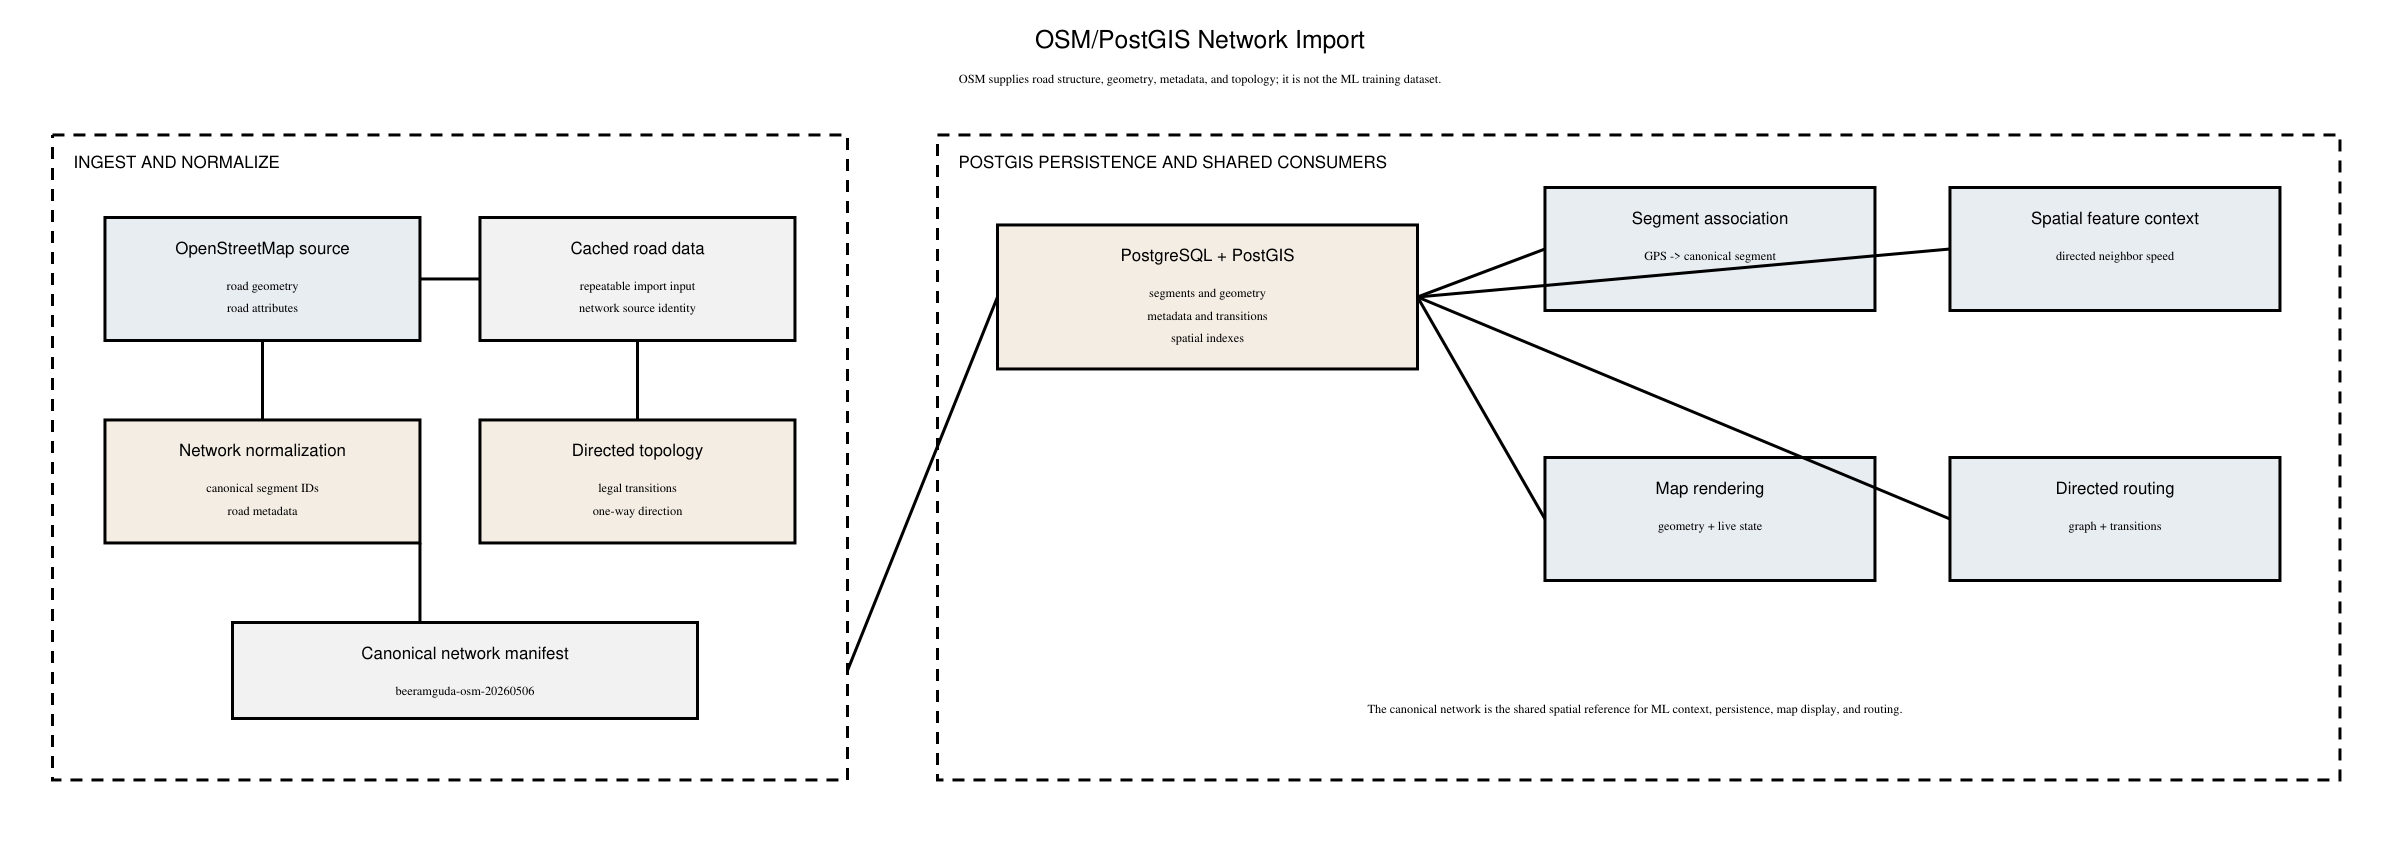
\includegraphics[width=0.9\textwidth,height=0.82\textheight,keepaspectratio]{fig_4_7.png}
\caption{OSM/PostGIS Network Import}
\label{fig:4-7}
\end{figure}

The Directed Road Network and Transitions is illustrated in Figure~\ref{fig:4-8}.\par

\begin{figure}[p]
\centering
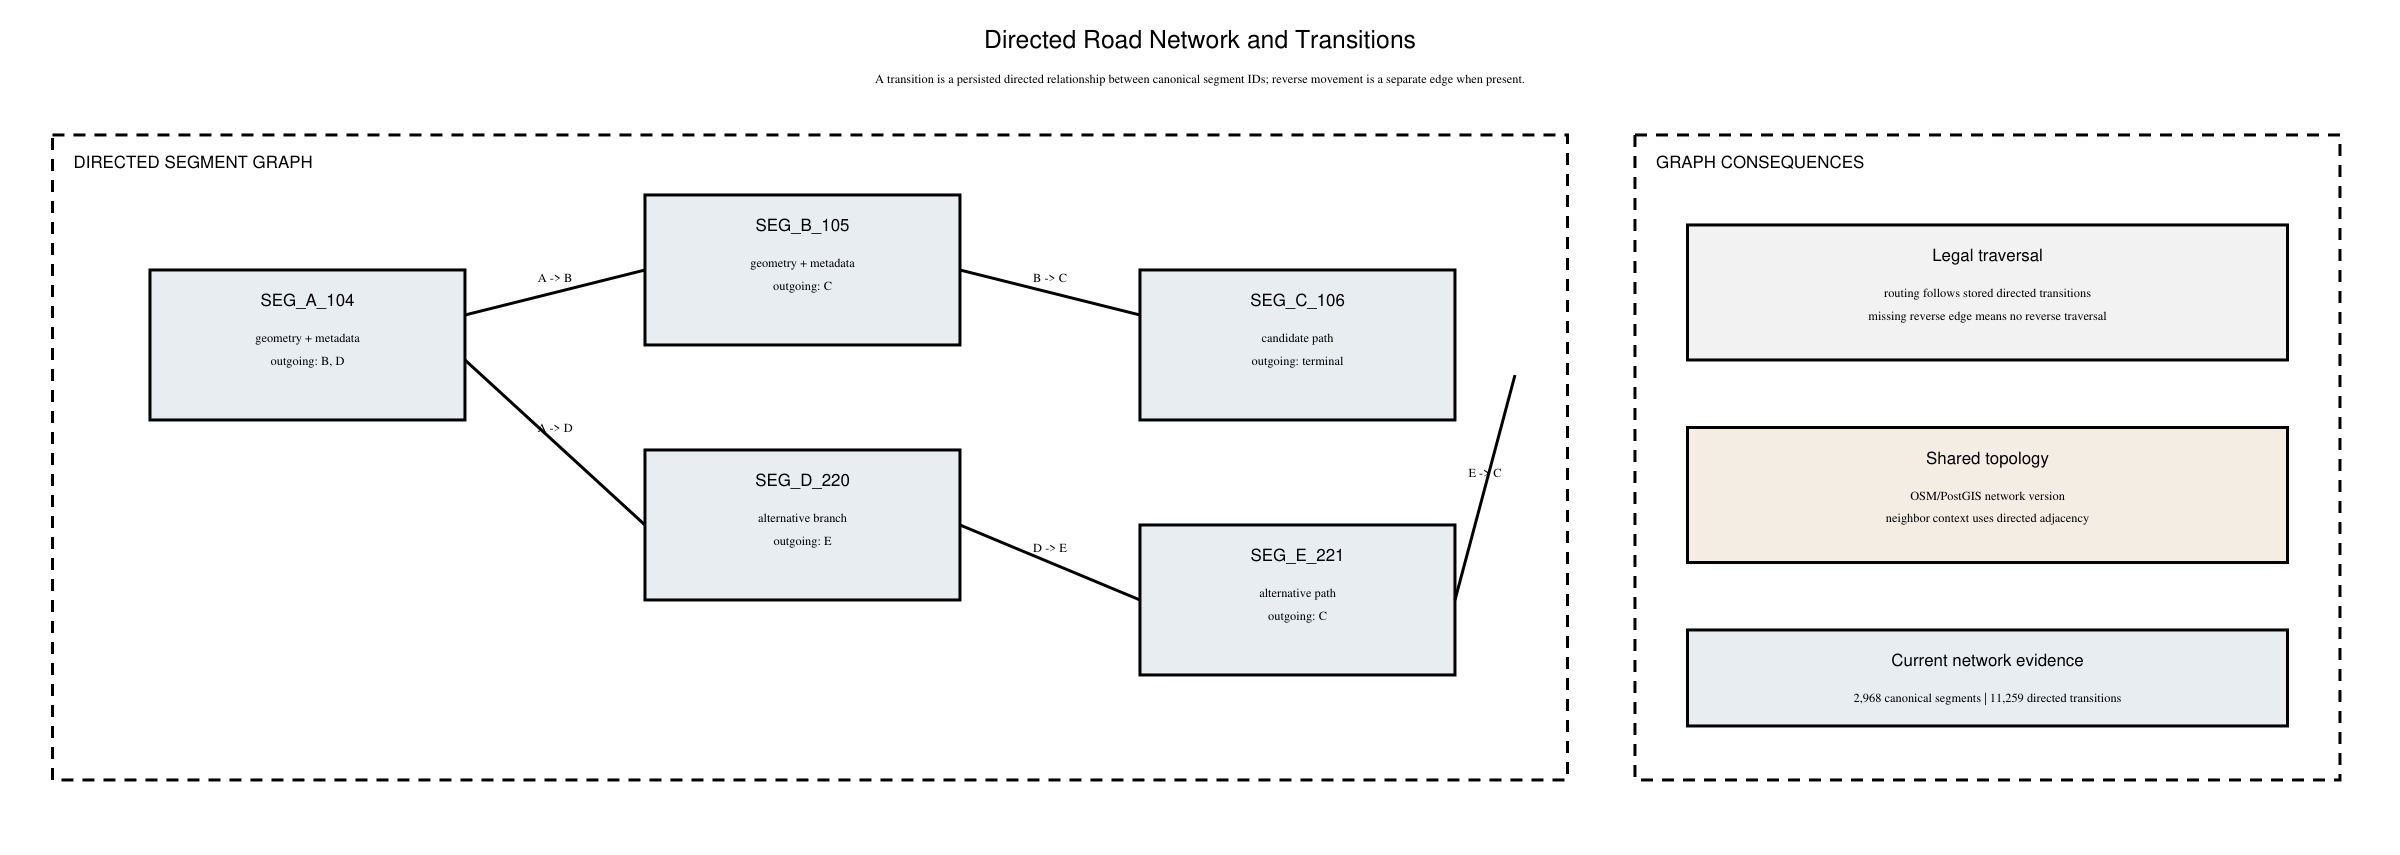
\includegraphics[width=0.9\textwidth,height=0.82\textheight,keepaspectratio]{fig_4_8.png}
\caption{Directed Road Network and Transitions}
\label{fig:4-8}
\end{figure}

The Backend Service and Repository Layers is illustrated in Figure~\ref{fig:4-9}.\par

\begin{figure}[p]
\centering
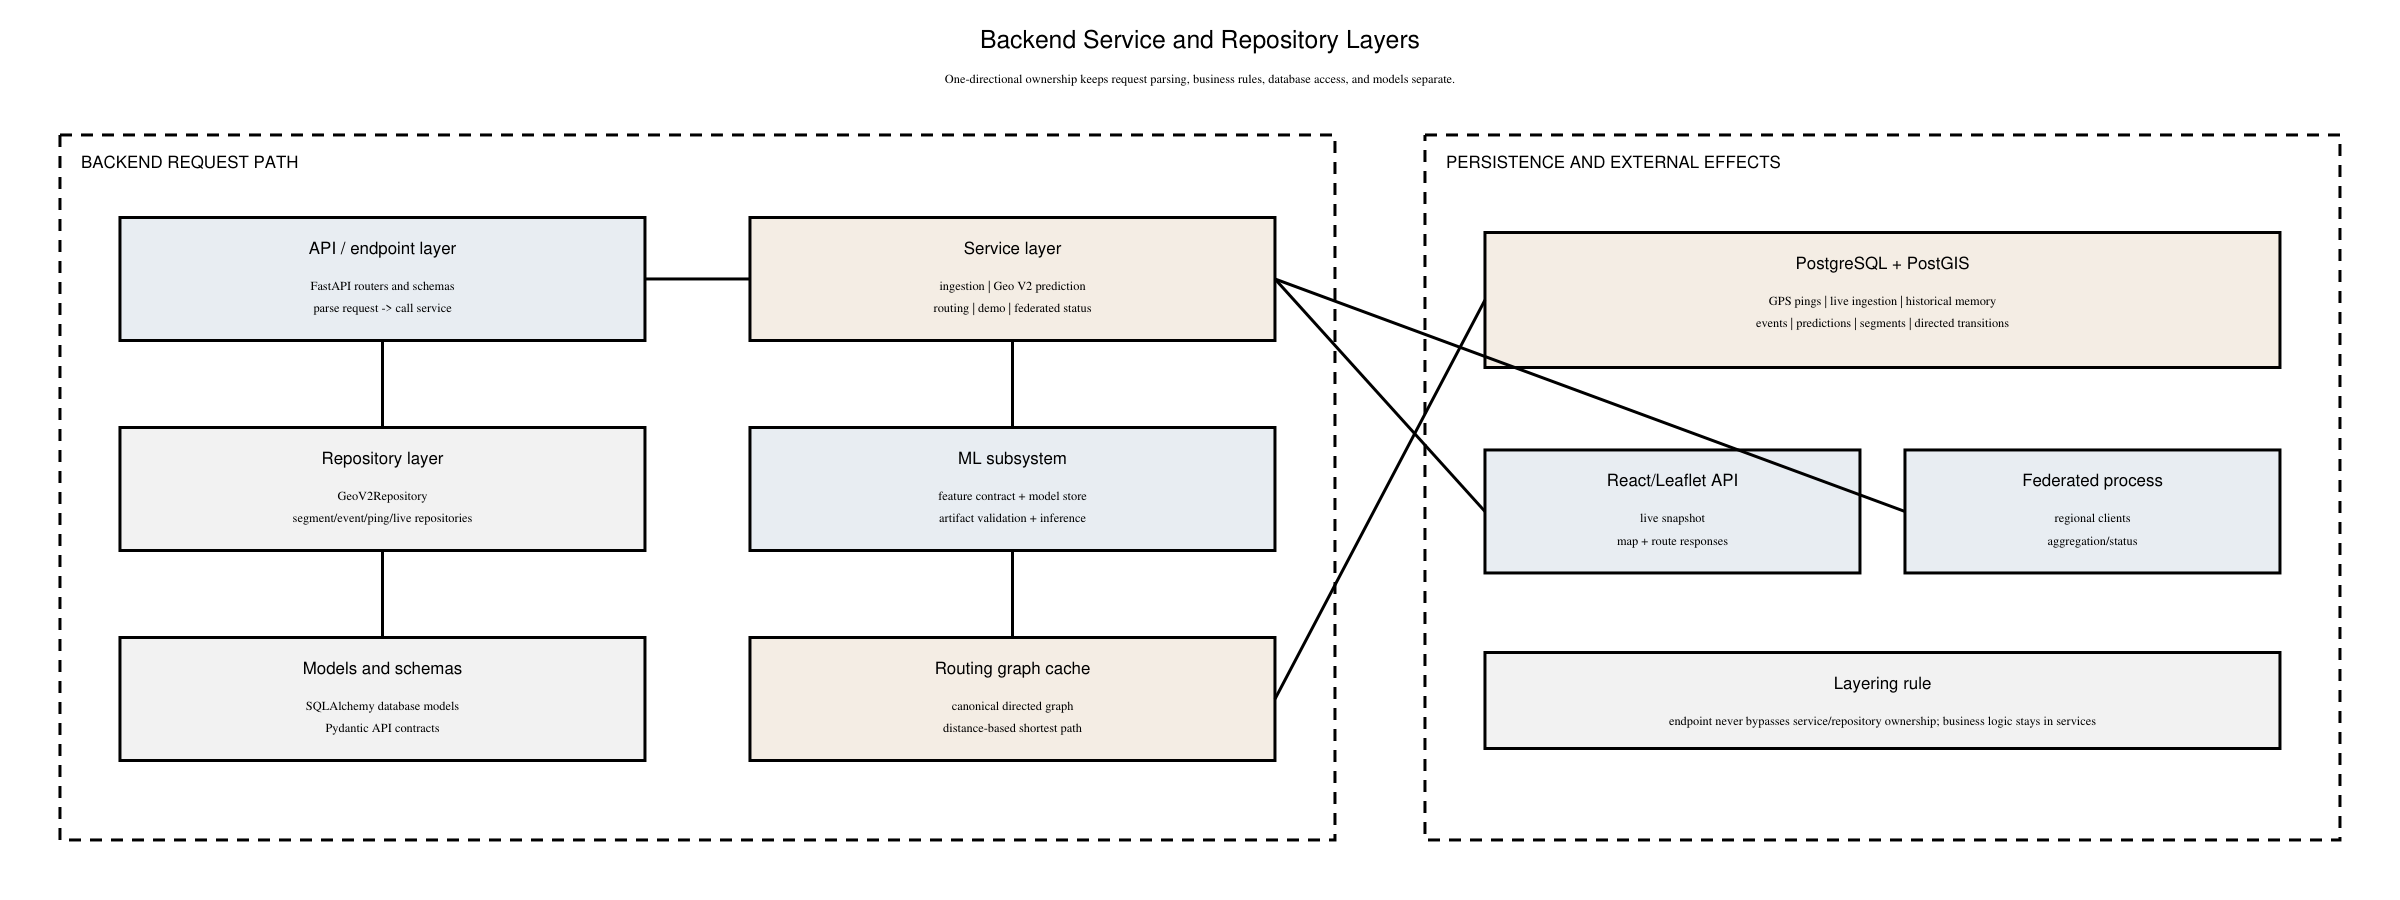
\includegraphics[width=0.9\textwidth,height=0.82\textheight,keepaspectratio]{fig_4_9.png}
\caption{Backend Service and Repository Layers}
\label{fig:4-9}
\end{figure}

The Frontend Map and API Interaction is illustrated in Figure~\ref{fig:4-10}.\par

\begin{figure}[p]
\centering
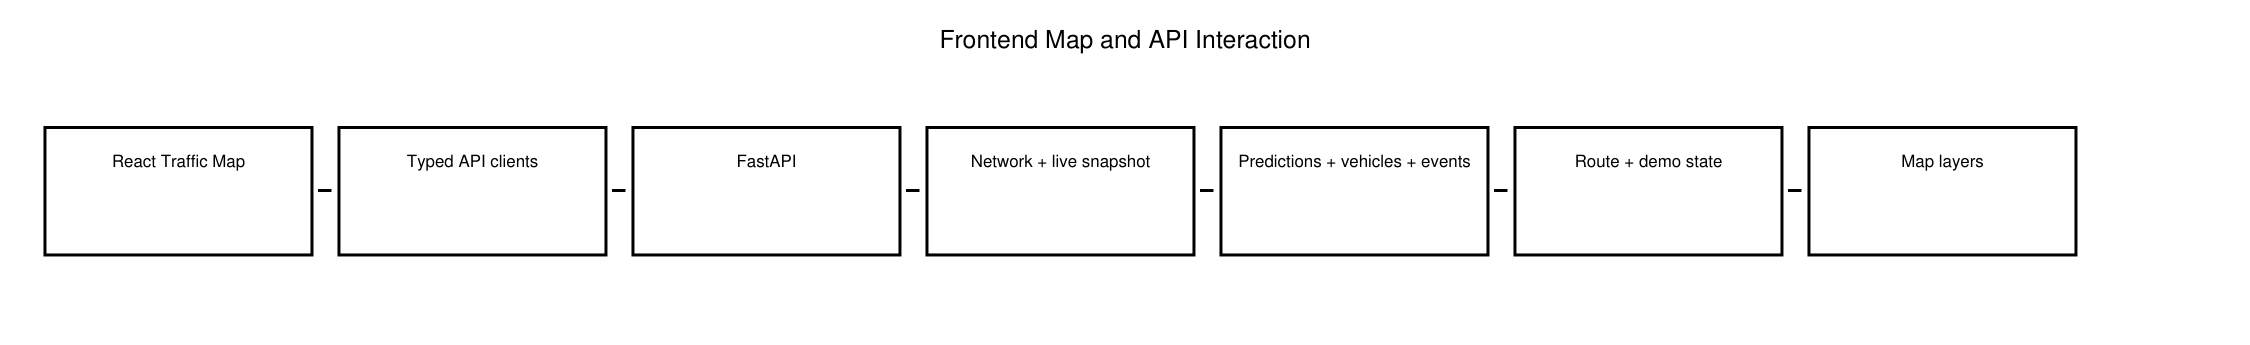
\includegraphics[width=0.9\textwidth,height=0.82\textheight,keepaspectratio]{fig_4_10.png}
\caption{Frontend Map and API Interaction}
\label{fig:4-10}
\end{figure}

The Directed Shortest-Path Routing is illustrated in Figure~\ref{fig:4-11}.\par

\begin{figure}[p]
\centering
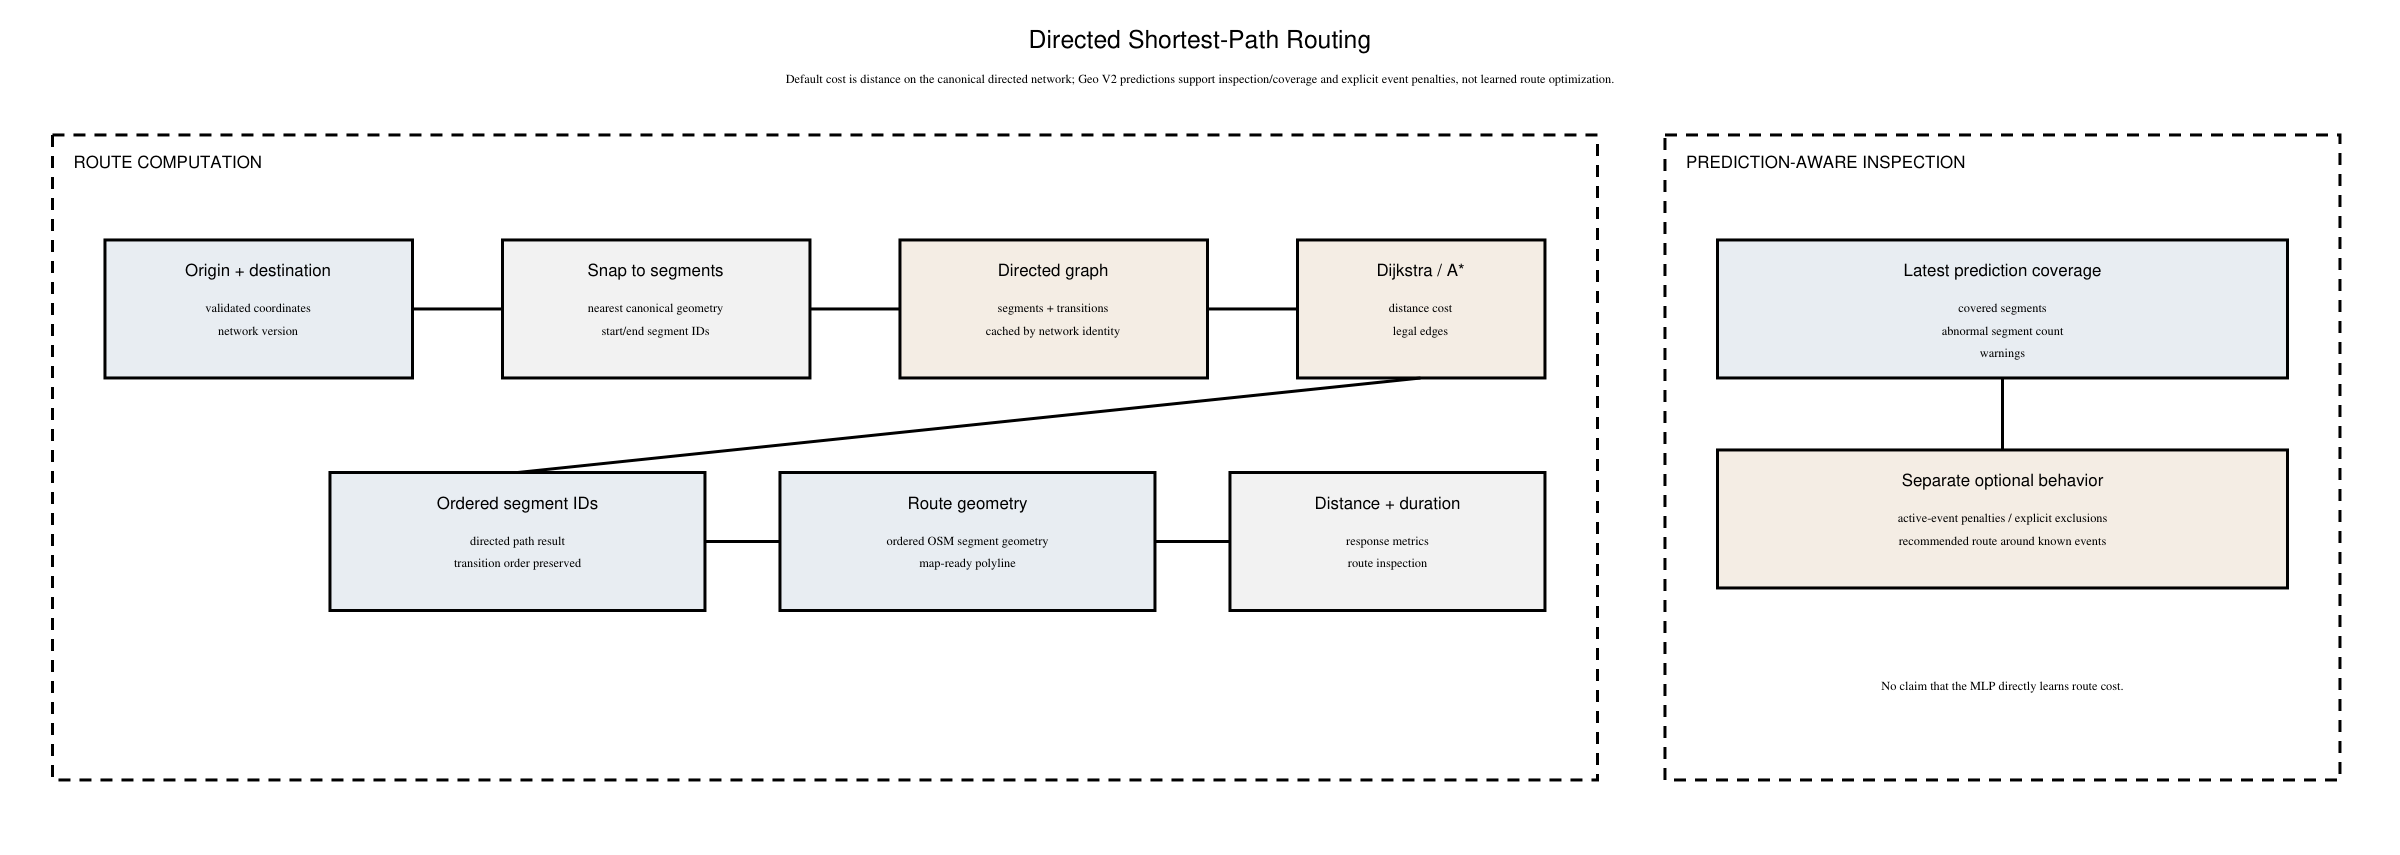
\includegraphics[width=0.9\textwidth,height=0.82\textheight,keepaspectratio]{fig_4_11.png}
\caption{Directed Shortest-Path Routing}
\label{fig:4-11}
\end{figure}

\chapter{IMPLEMENTATION}

\section{Data Ingestion and Processing}

The FedRouteAI implementation begins with the ingestion of GPS-based vehicle telemetry. The telemetry provides the geographic and movement information required to determine the position and traffic state of vehicles within the road network. The incoming observations are processed and associated with the corresponding road segments. This converts individual GPS observations into road-level information that can be used for traffic analysis. The use of a canonical road network ensures that traffic observations are represented consistently across the different components of the system. After road-segment association, the observations are aggregated to obtain segment-level traffic information. The aggregated information provides the basis for constructing the current traffic state of each road segment. Historical traffic information is also maintained as part of the processing pipeline. Current observations and historical information are combined during feature construction so that the machine learning model can use both present and previously observed traffic conditions. The implementation therefore follows the processing sequence:\par

\begin{center}\ttfamily\small GPS Telemetry  $\rightarrow$  Segment Association  $\rightarrow$  Traffic Aggregation  $\rightarrow$  Historical Traffic Processing  $\rightarrow$  Feature Construction\end{center}

This processing stage separates raw telemetry from the information eventually supplied to the machine learning model.\par

Table~\ref{tab:5-1} summarizes the Major Software Modules.\par

\begin{table}[htbp]
\centering
\caption{Major Software Modules}
\label{tab:5-1}
\renewcommand{\arraystretch}{1.25}
\begin{tabularx}{\textwidth}{@{}L L@{}}
\toprule
\textbf{Module} & \textbf{Role} \\
\midrule
app/api & Thin HTTP endpoints and request validation \\
app/services & Business logic and workflow orchestration \\
app/ml/geo\_v2 & Features, model store, and inference contract \\
app/repositories & Database and PostGIS access \\
frontend/src/pages/TrafficMap & Map, route, live controls, and inspection \\
scripts/geo\_v2 & Network import, dataset generation, replay, and validation \\
\bottomrule
\end{tabularx}
\end{table}

The Live GPS Ingestion Pipeline is illustrated in Figure~\ref{fig:5-1}.\par

\begin{figure}[p]
\centering
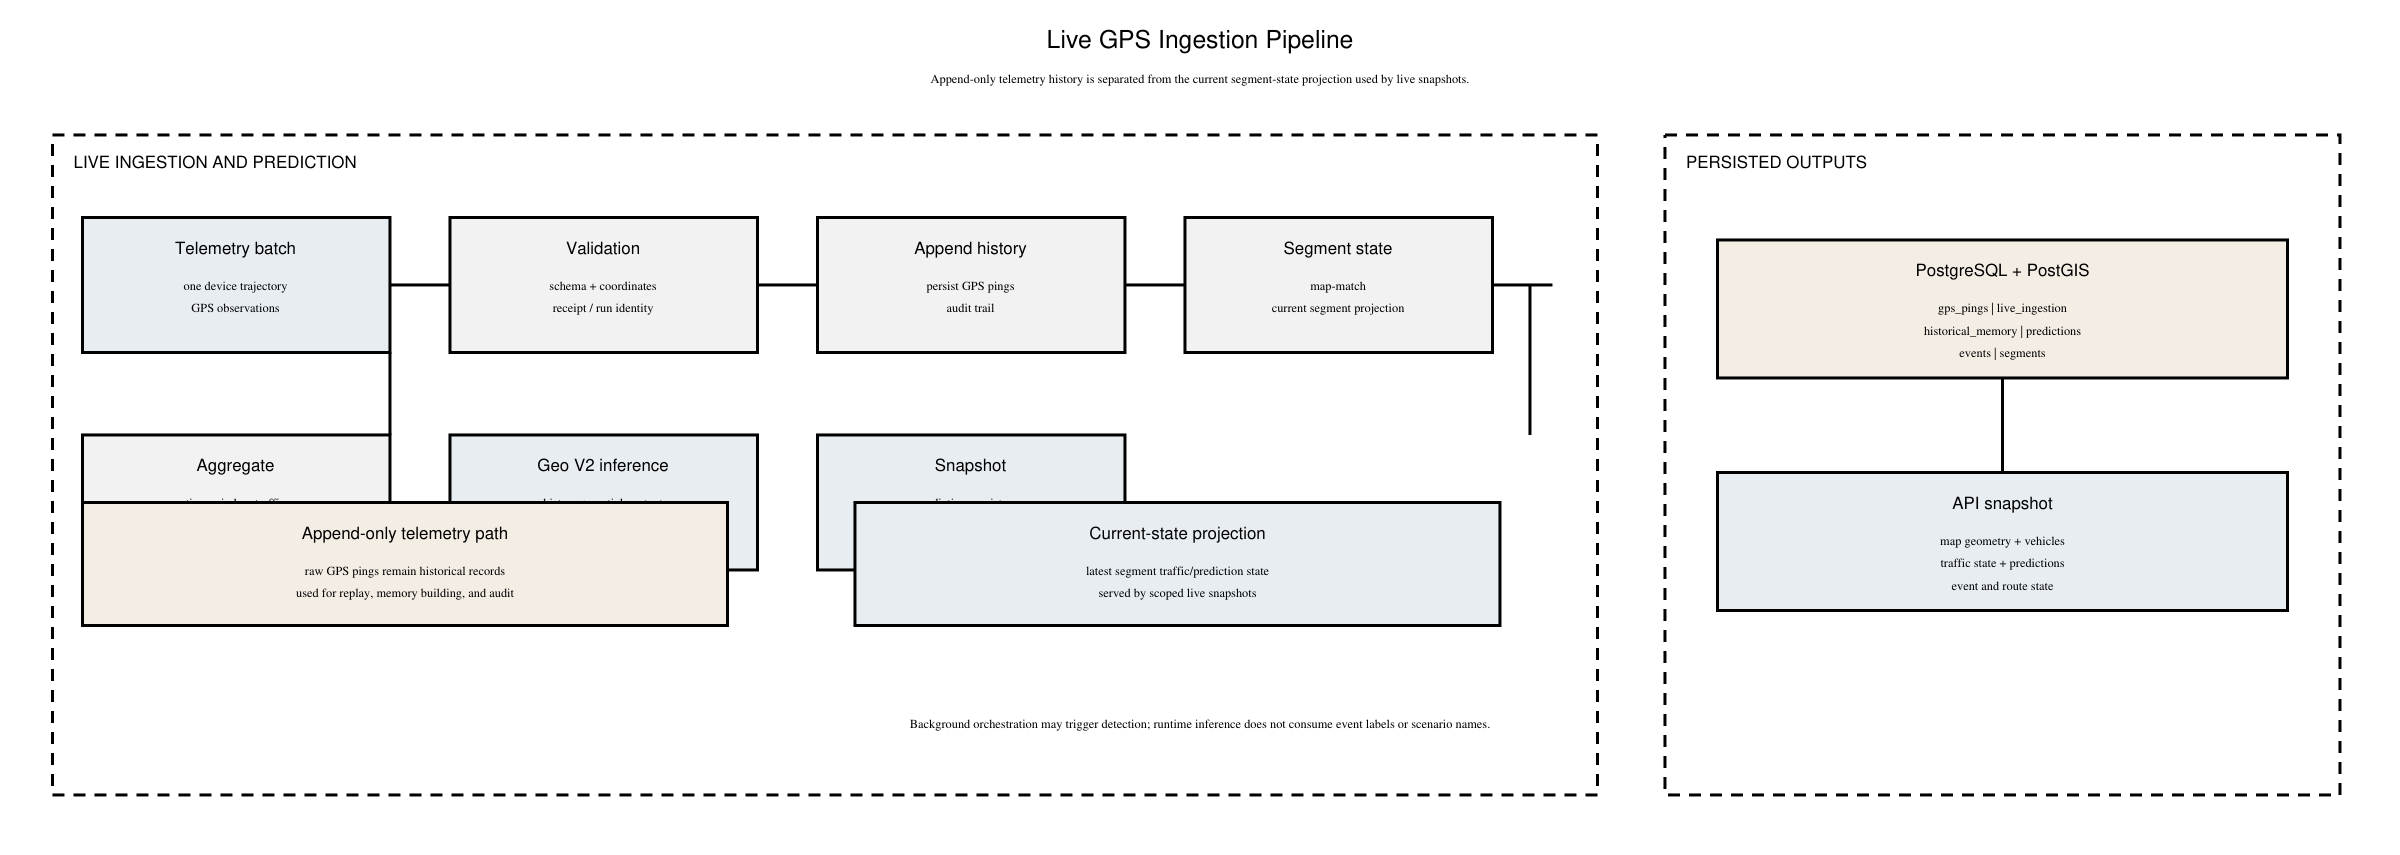
\includegraphics[width=0.9\textwidth,height=0.82\textheight,keepaspectratio]{fig_5_1.png}
\caption{Live GPS Ingestion Pipeline}
\label{fig:5-1}
\end{figure}

\section{Geo V2 Feature Construction}

The Geo V2 feature-construction component transforms the processed traffic information into the input representation required by the machine learning model. The implemented model uses a fixed set of 23 ordered features. These features represent the traffic, spatial, temporal~\cite{yang2022}, and historical information required by the trained MLP~\cite{goodfellow2016,bishop2006,paszke2019} model. The feature order is treated as a strict contract between model training and runtime inference. The feature-construction process obtains the required values from the processed traffic state, road-network information, and historical traffic memory. The resulting values are arranged in the defined order and subjected to the preprocessing required by the trained model. Maintaining the exact feature ordering is important because the model assigns a specific meaning to each input position. Therefore, the runtime feature vector must remain compatible with the representation used during training. The implementation also keeps prediction information separate from the feature inputs. The traffic-event~\cite{han2019} class or controlled demonstration selection is not directly supplied to the model as an input feature. This prevents the demonstration mechanism from becoming a source of ground-truth leakage during inference. The resulting process can be represented as:\par

\begin{center}\ttfamily\small Current Traffic State + Spatial Information + Historical Information  $\rightarrow$  Geo V2 Feature Builder  $\rightarrow$  23-Feature Vector  $\rightarrow$  Preprocessing\end{center}

\section{Federated Training}

The federated learning~\cite{mcmahan2017,kairouz2021,beutel2020} implementation represents eight regional clients participating in collaborative model training. Each client operates on its local regional training data and performs the required local model-training process. The local clients use the common model architecture and feature representation. After local training, the resulting model updates are provided to the aggregation process. FedAvg~\cite{mcmahan2017} provides the basic mechanism for combining the local model updates. The implementation also includes Adaptive FedAvg~\cite{yuan2024,lu2024} to provide adaptive weighting of regional contributions during aggregation. The aggregation process produces the global model that represents the combined learning from the participating regional clients. The resulting model artifact can subsequently be used by the inference pipeline. The federated training process can be summarized as:\par

\begin{center}\ttfamily\small Regional Data  $\rightarrow$  Local Client Training  $\rightarrow$  Local Model Updates  $\rightarrow$  Federated Aggregation  $\rightarrow$  Global Model\end{center}

The use of federated training reduces the requirement to centralize the complete raw training datasets. However, the current implementation does not provide formal differential privacy~\cite{liu2020}~\cite{dwork2014,abadi2016,wei2020} or secure aggregation~\cite{kairouz2021,shokri2015}.\par

\section{Model Inference}

The trained global model is used for traffic-event prediction during runtime. FedRouteAI uses a Multilayer Perceptron (MLP) classifier that receives the processed 23-feature Geo V2 representation as input. Before inference, the runtime feature vector is prepared according to the same feature ordering and preprocessing requirements used during training. This ensures compatibility between the runtime feature-construction process and the trained model artifact. The MLP processes the feature vector and produces the predicted traffic-event class supported by the model. The prediction is then passed to the persistence and API layers. The inference process does not directly use controlled demonstration labels. Scenario selection used for demonstration purposes remains separate from the model's input and prediction process. The runtime inference flow is therefore:\par

\begin{center}\ttfamily\small Processed Traffic Data  $\rightarrow$  Geo V2 Features  $\rightarrow$  Preprocessing  $\rightarrow$  MLP Model  $\rightarrow$  Traffic-Event Prediction\end{center}

This separation provides a clear boundary between feature construction and model inference and allows the model component to be evaluated independently.\par

\section{API and Persistence}

The backend provides the application services required to connect the traffic-processing and machine-learning components with the frontend. FastAPI~\cite{fastapi} is used to expose the required API operations. The backend receives and processes application requests, accesses the spatial database, performs the required service operations, and returns traffic and prediction information to the frontend. Model predictions generated during runtime are persisted so that they can be retrieved by the application. The persistence layer also maintains the spatial and traffic information required for visualization and other application operations. The backend follows a modular organization in which API handling, service logic, machine learning, processing, and database access are separated according to their responsibilities. This organization supports maintainability and testing. The application flow can be summarized as:\par

\begin{center}\ttfamily\small Processing / Model  $\rightarrow$  Prediction Persistence  $\rightarrow$  FastAPI  $\rightarrow$  Frontend\end{center}

The API therefore acts as the interface between the backend processing system and the web-based user interface.\par

\section{Frontend and Visualization}

The FedRouteAI frontend is implemented using React~\cite{react_leaflet} and provides the user-facing interface for the traffic-intelligence system. The frontend communicates with the backend through the defined APIs and retrieves the road-network, traffic, prediction, vehicle, and routing information required for visualization. An interactive map is used to represent the spatial information. The map allows users to view the road network and observe traffic-related information in its geographic context. Vehicle movement and traffic-event predictions can also be represented through the interface. The frontend provides a visual separation between the different types of information generated by the system. Traffic observations, predictions, vehicle movement, and routes can therefore be inspected through the same application without requiring direct access to the underlying database or machine learning components. The frontend workflow can be represented as:\par

\begin{center}\ttfamily\small User  $\rightarrow$  React Interface  $\rightarrow$  API  $\rightarrow$  Backend  $\rightarrow$  Database / ML / Processing  $\rightarrow$  API  $\rightarrow$  Map Visualization\end{center}

This architecture keeps the presentation layer separate from the underlying processing and machine-learning implementation.\par

\section{Routing and Demonstration}

The routing component operates on the directed road network stored in the spatial database. It accepts an origin and destination and identifies the corresponding locations within the available road network. Dijkstra~\cite{dijkstra1959}'s algorithm is used to compute the shortest path through the directed network. The resulting route is returned by the backend and displayed on the frontend map. The current routing implementation is distance-based. Traffic-event predictions are not currently incorporated into the route cost. Therefore, the system should not be interpreted as providing a fully traffic-aware routing optimization system. FedRouteAI also includes controlled traffic demonstrations for illustrating different traffic conditions. These demonstrations may represent scenarios such as Normal, Congestion, and Accident. Their purpose is to provide a controlled way of displaying system behavior and validating the application workflow. The demonstration mechanism is kept separate from the machine learning inference process. Selecting a demonstration scenario does not directly provide the corresponding event label to the model. This separation ensures that demonstration behavior is not incorrectly presented as model ground truth. The implementation therefore maintains two related but independent workflows:\par

\begin{center}\ttfamily\small Traffic Prediction: \\ Telemetry  $\rightarrow$  Traffic Processing  $\rightarrow$  Geo V2  $\rightarrow$  MLP  $\rightarrow$  Prediction\end{center}

\begin{center}\ttfamily\small Routing/Demonstration: \\ Road Network  $\rightarrow$  Route Computation / Controlled Scenario  $\rightarrow$  Frontend Visualization\end{center}

This separation provides a clear distinction between machine-learning output, route computation, and controlled demonstration behavior.\par

Table~\ref{tab:5-2} summarizes the Model Configuration.\par

\begin{table}[htbp]
\centering
\caption{Model Configuration}
\label{tab:5-2}
\renewcommand{\arraystretch}{1.25}
\begin{tabularx}{\textwidth}{@{}L L@{}}
\toprule
\textbf{Property} & \textbf{Verified value} \\
\midrule
Runtime model & GeoV2MLP \\
Output classes & 8 \\
Input feature count & 23 \\
Feature version & geo-v2-history\_spatial\_strong-23-v2 \\
Training rounds & 50 maximum; checkpoint round 45 \\
Local epochs & 2 \\
Dropout & 0.2 in runtime architecture \\
Inference mode & Label-free feature input \\
\bottomrule
\end{tabularx}
\end{table}

Table~\ref{tab:5-3} summarizes the Demonstration Controls.\par

\begin{table}[htbp]
\centering
\caption{Demonstration Controls}
\label{tab:5-3}
\renewcommand{\arraystretch}{1.25}
\begin{tabularx}{\textwidth}{@{}L L@{}}
\toprule
\textbf{Control} & \textbf{Behavior} \\
\midrule
Normal & Baseline route-bound traffic behavior \\
Congestion & Controlled congestion-like route behavior \\
Accident & Controlled accident-like route disturbance \\
Minimum route & Approximately 1.5 km \\
Route binding & Ordered directed segment IDs supplied by route calculation \\
Truth handling & Scenario metadata excluded from model features \\
\bottomrule
\end{tabularx}
\end{table}

The Frozen Geo V2 MLP Inference is illustrated in Figure~\ref{fig:5-2}.\par

\begin{figure}[p]
\centering
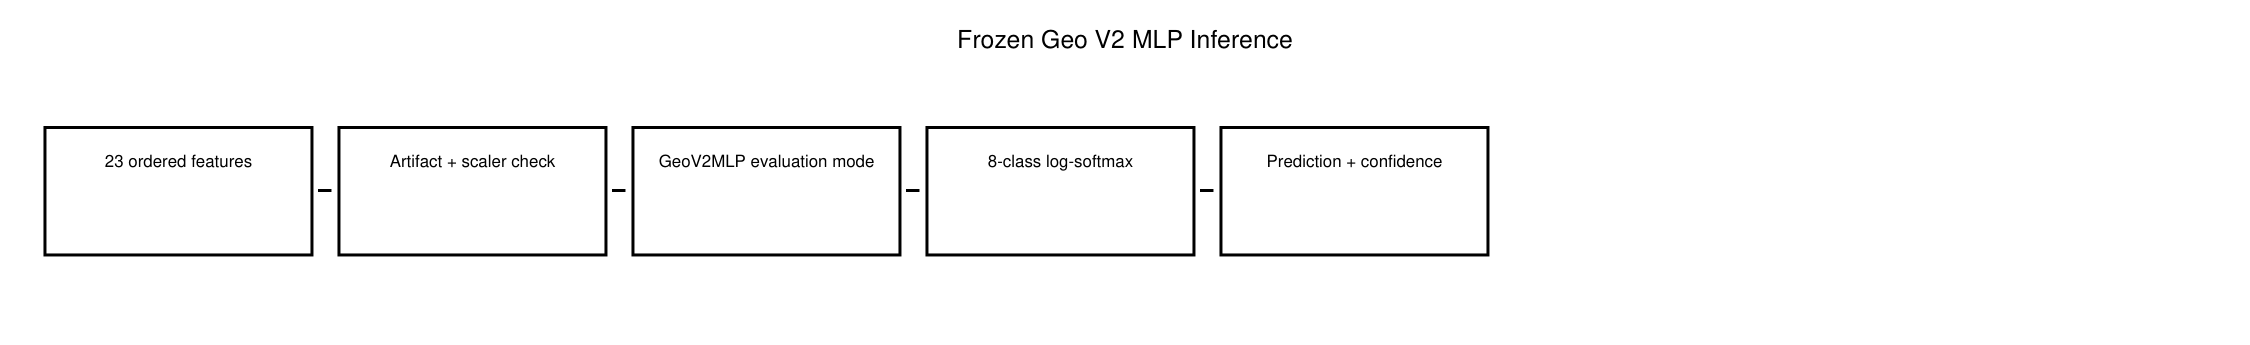
\includegraphics[width=0.9\textwidth,height=0.82\textheight,keepaspectratio]{fig_5_2.png}
\caption{Frozen Geo V2 MLP Inference}
\label{fig:5-2}
\end{figure}

The Dynamic Traffic Map is illustrated in Figure~\ref{fig:5-3}.\par

\begin{figure}[p]
\centering
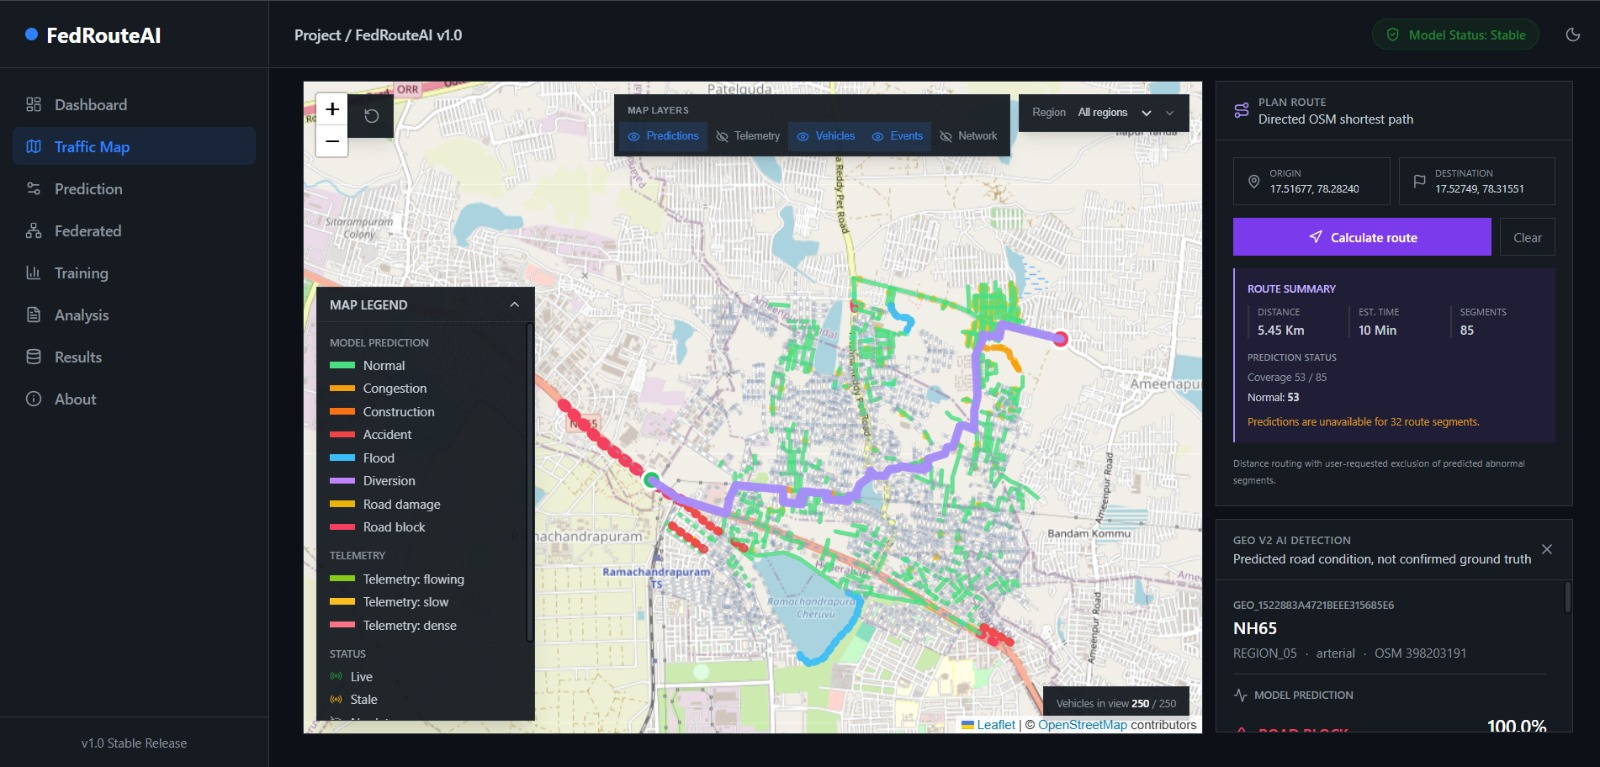
\includegraphics[width=0.9\textwidth,height=0.82\textheight,keepaspectratio]{fig_5_3.jpeg}
\caption{Dynamic Traffic Map}
\label{fig:5-3}
\end{figure}

The Moving Vehicle Visualization is illustrated in Figure~\ref{fig:5-4}.\par

\begin{figure}[p]
\centering
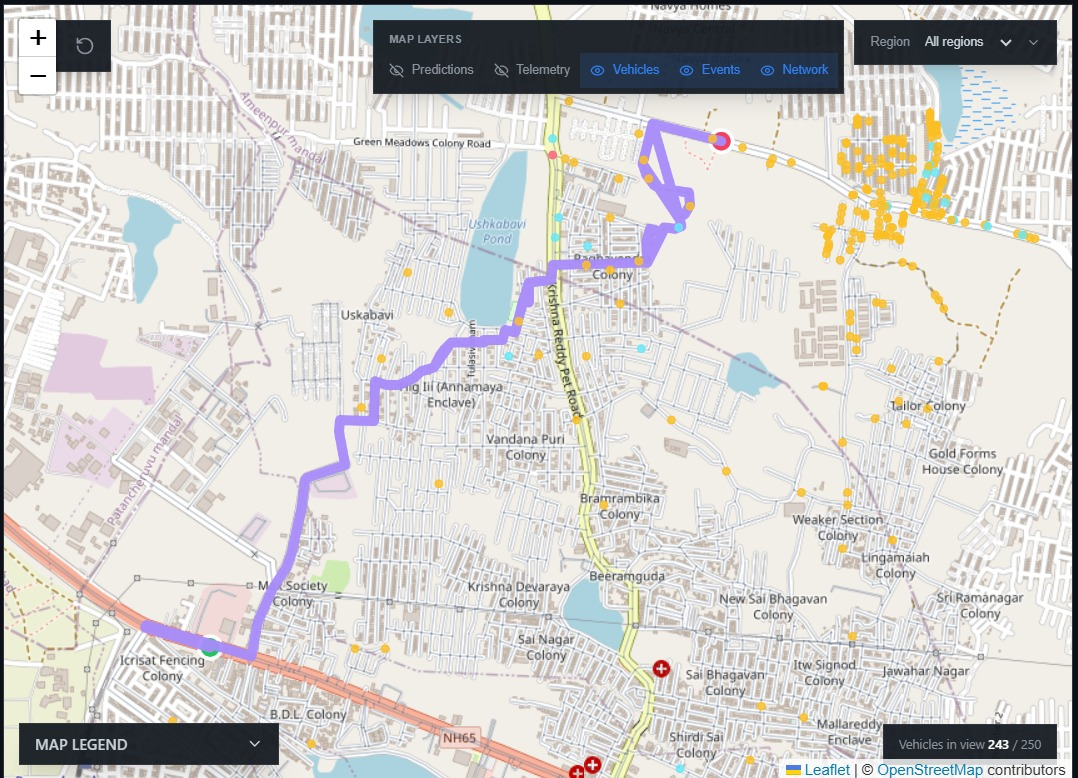
\includegraphics[width=0.9\textwidth,height=0.82\textheight,keepaspectratio]{fig_5_4.jpeg}
\caption{Moving Vehicle Visualization}
\label{fig:5-4}
\end{figure}

The Route-Bound Demonstration Flow is illustrated in Figure~\ref{fig:5-5}.\par

\begin{figure}[p]
\centering
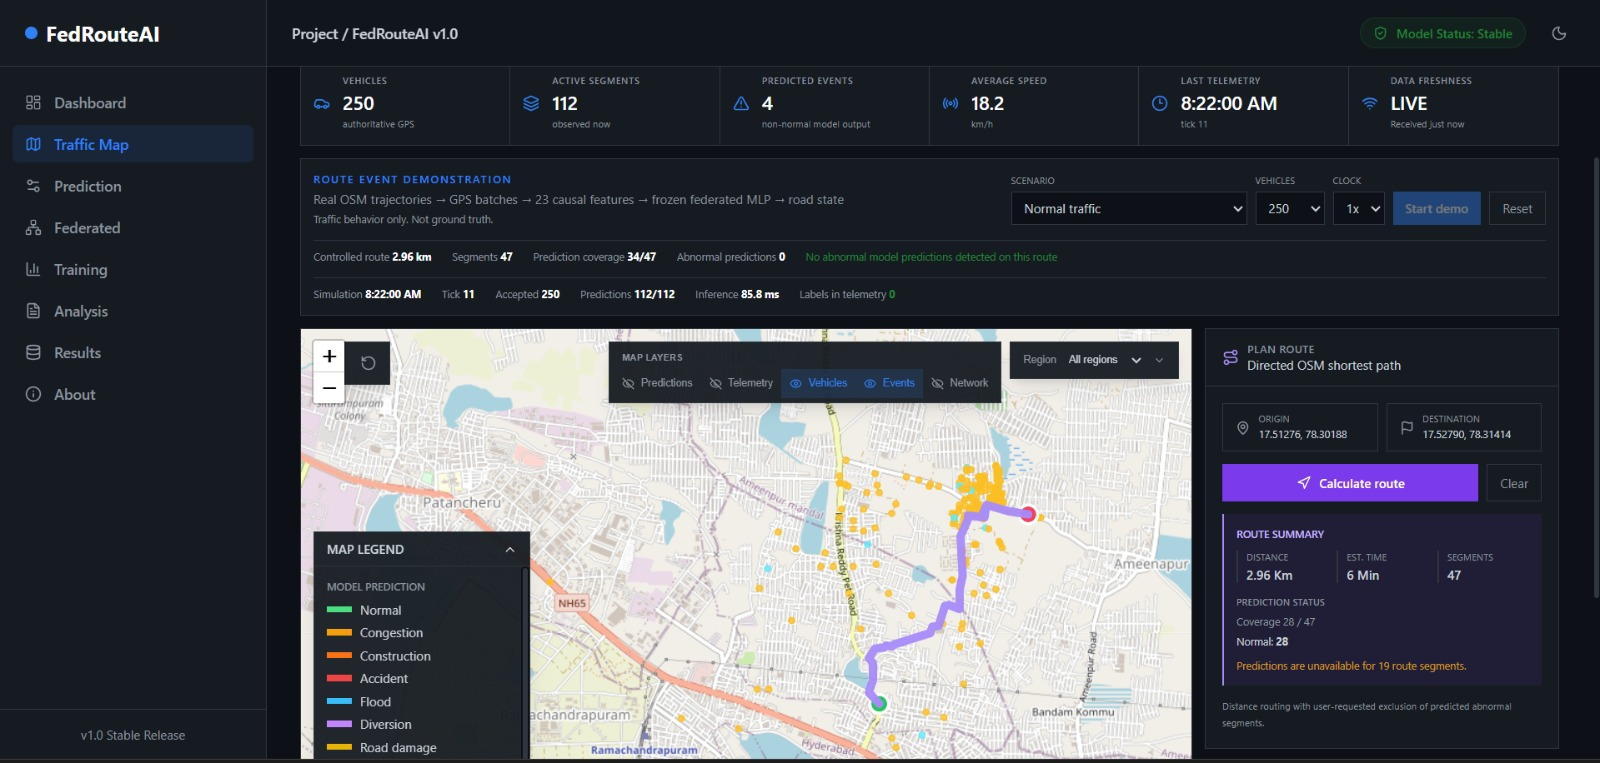
\includegraphics[width=0.9\textwidth,height=0.82\textheight,keepaspectratio]{fig_5_5.jpeg}
\caption{Route-Bound Demonstration Flow}
\label{fig:5-5}
\end{figure}

The Normal Traffic Demonstration is illustrated in Figure~\ref{fig:5-6}.\par

\begin{figure}[p]
\centering
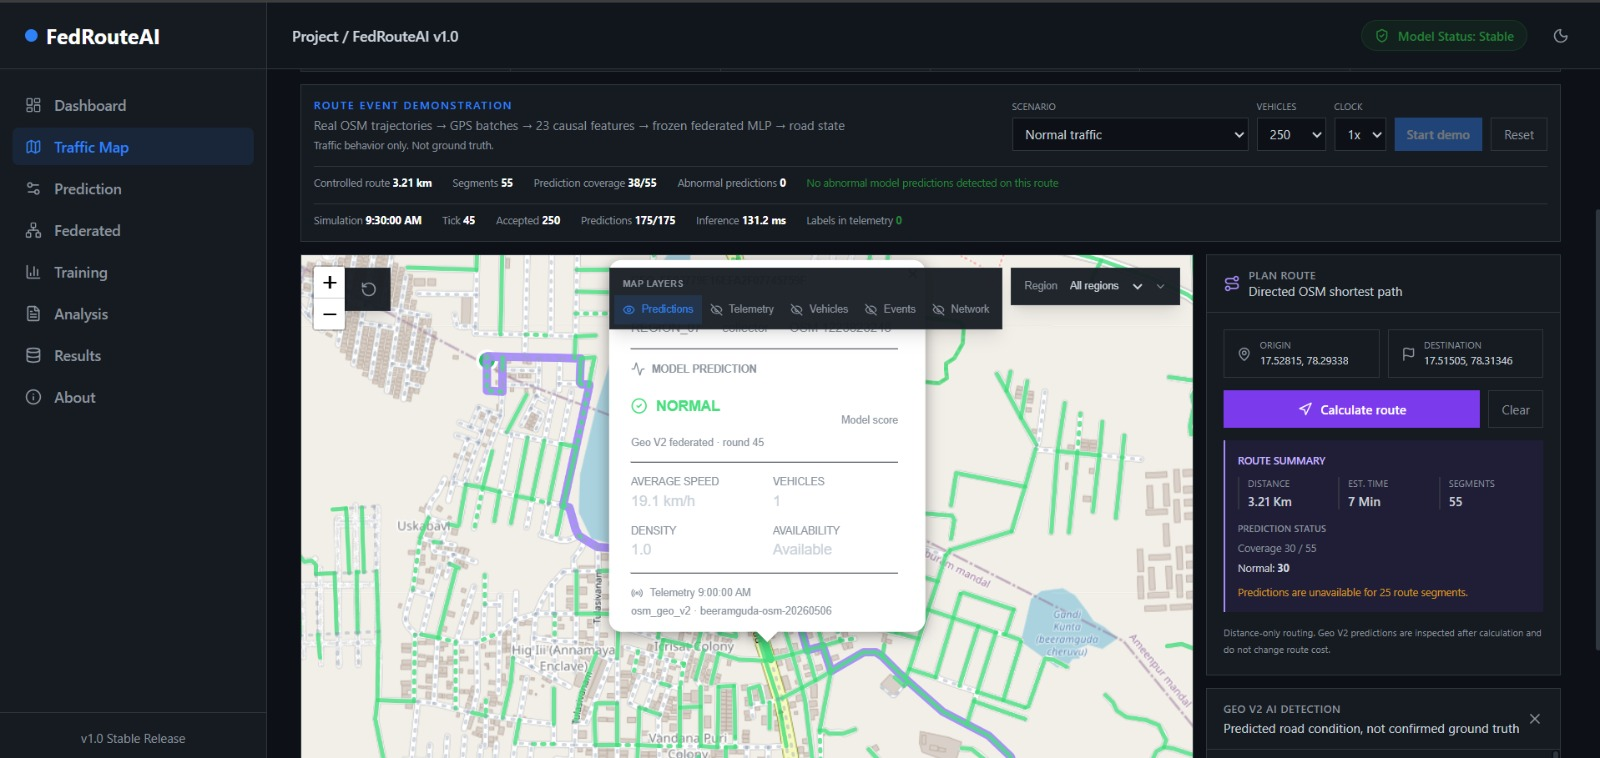
\includegraphics[width=0.9\textwidth,height=0.82\textheight,keepaspectratio]{fig_5_6.jpeg}
\caption{Normal Traffic Demonstration}
\label{fig:5-6}
\end{figure}

The Congestion and Accident Demonstrations is illustrated in Figure~\ref{fig:5-7}.\par

\begin{figure}[p]
\centering
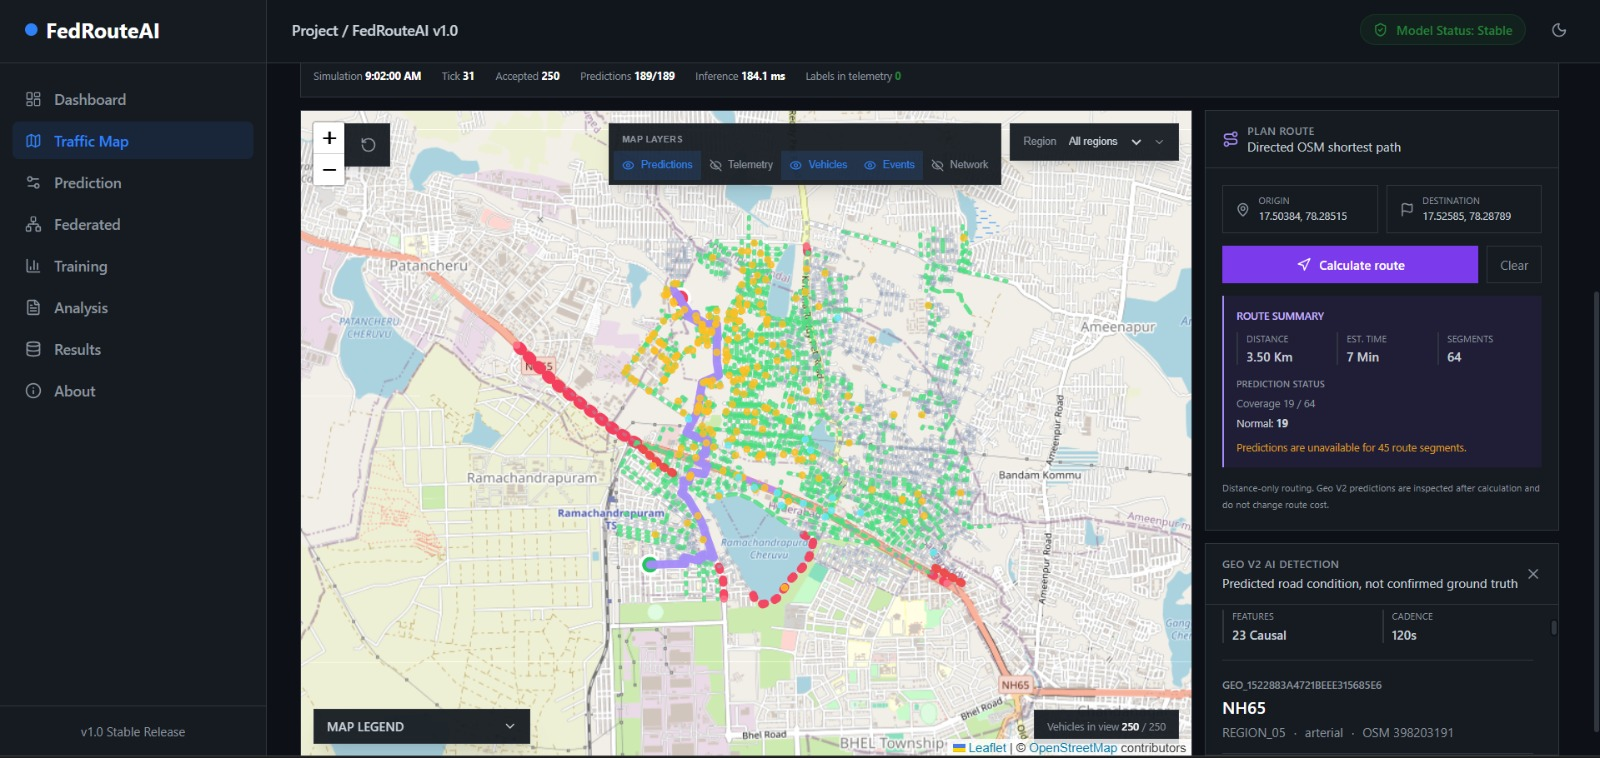
\includegraphics[width=0.9\textwidth,height=0.82\textheight,keepaspectratio]{fig_5_7.jpeg}
\caption{Congestion and Accident Demonstrations}
\label{fig:5-7}
\end{figure}

\chapter{TESTING AND VALIDATION}

\section{Testing Strategy}

Testing is an important part of the FedRouteAI implementation because the system contains multiple interconnected components, including telemetry processing, Geo V2 feature construction, federated learning~\cite{mcmahan2017,kairouz2021,beutel2020}, model inference, spatial processing, backend APIs, frontend visualization, and routing. The testing process is designed to verify the correctness of individual components as well as their interaction within the complete application. Testing covers backend services, machine learning functionality, spatial processing, routing, frontend functionality, and runtime behavior. The testing approach includes unit and service-level tests, API testing, feature-validation tests, model-artifact validation, routing tests, ingestion tests, frontend tests, build validation, and runtime checks. The main objective is to ensure that the implemented components operate according to their intended functionality and that the interfaces between components remain consistent.\par

The Model Validation Results is illustrated in Figure~\ref{fig:6-1}.\par

\begin{figure}[p]
\centering
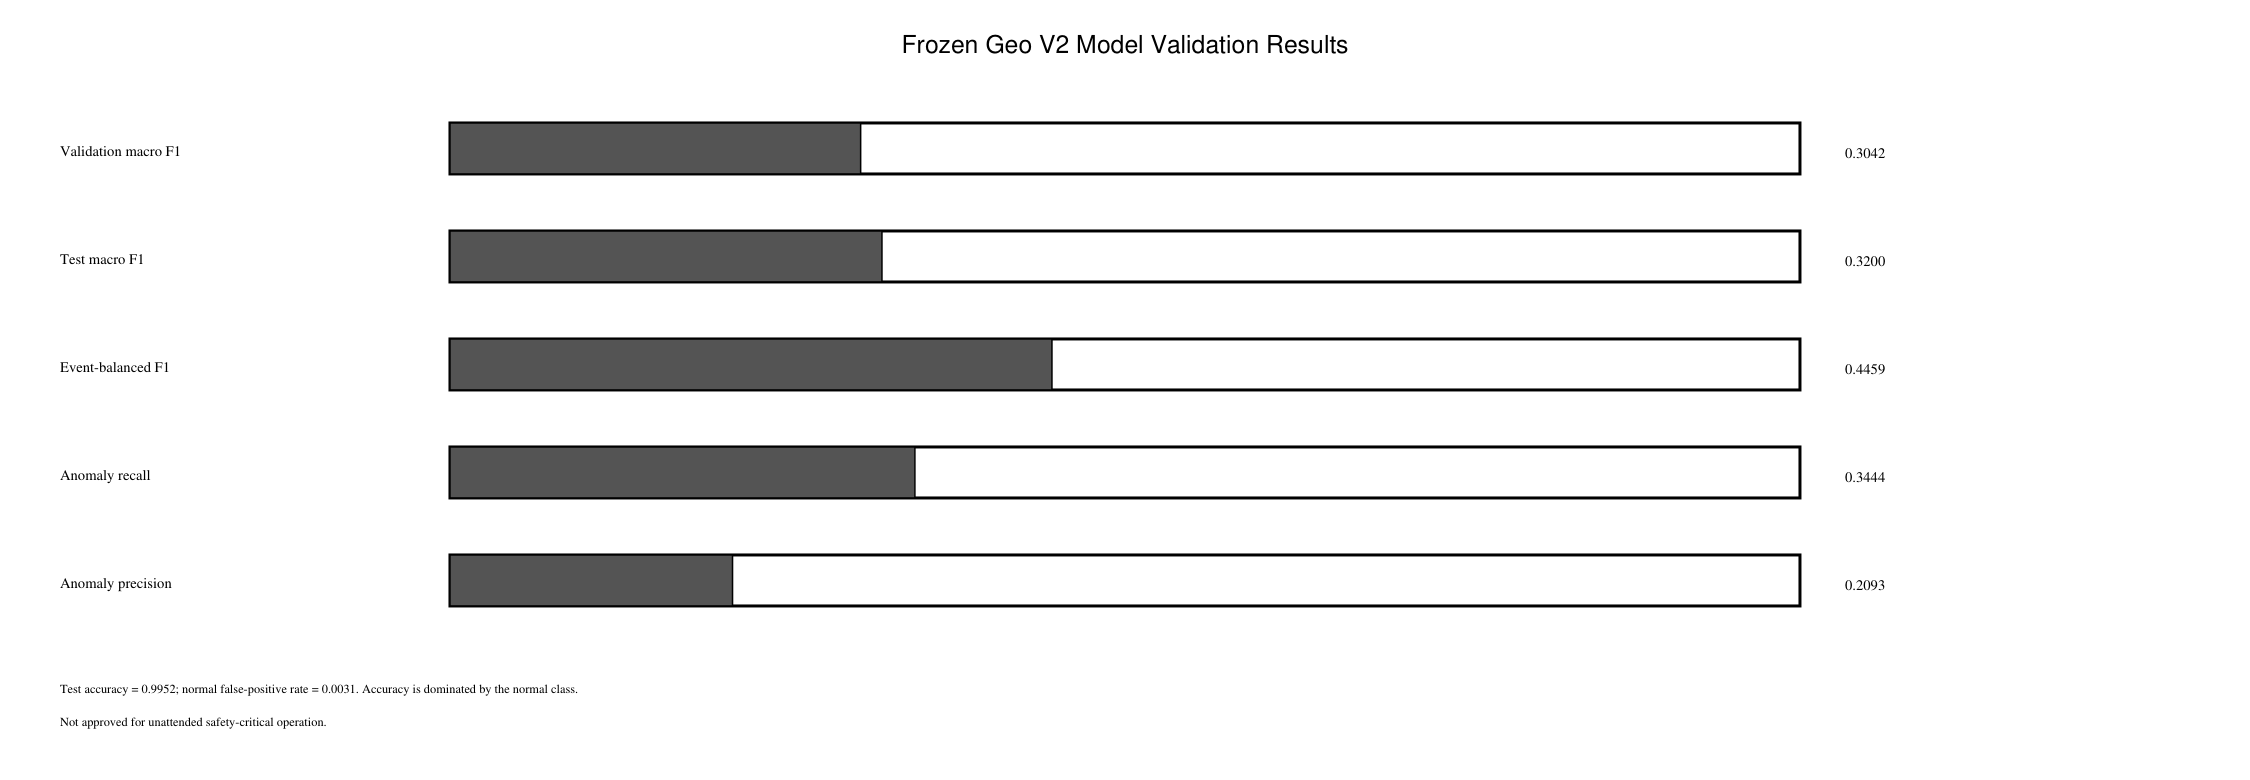
\includegraphics[width=0.9\textwidth,height=0.82\textheight,keepaspectratio]{fig_6_1.png}
\caption{Model Validation Results}
\label{fig:6-1}
\end{figure}

\section{Backend and Service Testing}

Backend testing verifies the functionality of services responsible for telemetry processing, traffic aggregation, feature construction, model inference, persistence, and API operations. The backend test suite covers the major application services and checks whether individual components produce the expected results for supported inputs. API testing verifies communication~\cite{zhou2019,wang2020,khan2020} between the frontend and backend by checking that required endpoints respond correctly and return information consistent with the application data. The testing process also verifies error handling and input validation to ensure that invalid or unexpected requests do not cause unintended behavior. The completed backend test suite provides evidence that the implemented backend services operate as expected within the scope of the prototype.\par

\section{Geo V2 and Feature Validation}

The Geo V2 feature pipeline is tested separately because the machine learning model depends on the exact feature representation used during training. The feature-validation tests verify that the required 23 features are generated in the correct order and that the resulting representation is compatible with the trained model~\cite{goodfellow2016,bishop2006,paszke2019}. The tests also verify the handling of traffic, spatial, temporal~\cite{yang2022}, and historical information used during feature construction. This helps identify inconsistencies between the training-time and runtime feature pipelines. Feature validation is particularly important because an incorrect feature order or preprocessing operation can result in model-serving incompatibility even when the model artifact itself is valid. The validation process therefore treats the Geo V2 feature representation as a formal interface between the traffic-processing pipeline and the machine learning model.\par

\section{Model Validation}

Model validation evaluates the trained MLP traffic-event~\cite{han2019} classifier using the available validation and test data. The model achieved a Validation Macro F1 of 0.3042, Test Macro F1 of 0.3200, Event-balanced Macro F1 of 0.4459, Anomaly Recall~\cite{hendrycks2017} of 0.3444, Anomaly Precision of 0.2093, and a Normal False Positive Rate of 0.0031. These results indicate that the model can perform traffic-event classification within the experimental environment, although performance varies across traffic-event categories due to class imbalance~\cite{lu2024}. Macro-averaged and event-balanced metrics therefore provide a more informative assessment across the supported classes. The stored model was also validated for successful loading and compatibility with the expected 23-feature input representation. Overall, the results represent prototype-level validation based on the available experimental dataset and should not be interpreted as production-level traffic-event detection accuracy.\par

\section{Routing and Integration Testing}

The routing component is tested independently to verify that origin and destination points can be processed against the directed road network and that Dijkstra~\cite{dijkstra1959}'s algorithm generates a valid shortest path when available. The resulting route is checked to ensure that it follows the directed road network. Integration testing verifies the interaction between major application components, including telemetry processing, feature construction, model inference, prediction persistence, API access, and frontend map visualization. Routing tests are kept separate from model evaluation because the current routing implementation is distance-based and does not use predicted traffic events as dynamic route costs.\par

\section{Frontend and Runtime Validation}

Frontend testing verifies the main user-interface components and their interaction with the backend APIs. The frontend validation covers the display of the road network, vehicle information, traffic conditions, prediction information, route visualization, and other supported application views. The frontend test suite includes focused tests for the implemented application components. Build validation is also performed to ensure that the frontend can be compiled successfully. Runtime validation checks the complete application in its execution environment. This includes starting the required services, connecting the frontend and backend, accessing the database, loading the model artifact, and verifying the main application workflow. The reported testing evidence includes 117 backend tests and 17 focused frontend tests, together with the other feature, artifact, routing, ingestion, build, and runtime validation activities documented for the project. These tests provide evidence that the major components of the implemented prototype can operate together under the tested environment.\par

\section{Performance Evaluation}

Performance evaluation is used to understand the computational behavior of the implemented model and application components. The model inference measurement reported for the project is approximately 0.414 ms per inference under the measured experimental conditions. This measurement represents isolated warmed model inference and should not be interpreted as the end-to-end~\cite{projsrc} throughput of the complete application. The complete application involves additional operations such as telemetry processing, spatial operations, database access, API communication, and frontend rendering. These operations contribute to overall response time and are therefore distinct from the isolated model-inference measurement. Performance results should also be interpreted in relation to the hardware and software environment in which the measurements were obtained. The current evaluation is intended to demonstrate prototype-level computational feasibility rather than production-scale capacity.\par

\section{Testing Results}

The testing activities provide evidence that the major FedRouteAI components satisfy their intended prototype-level functionality. The backend services, API operations, feature-construction pipeline, model artifact, routing functionality, frontend components, build process, and runtime workflow were tested using the available test and validation procedures. The machine learning evaluation demonstrates that the trained MLP can perform traffic-event classification on the experimental dataset. At the same time, the reported metrics show that minority-event detection remains a limitation, particularly in terms of anomaly precision and recall. The testing results therefore support the technical feasibility of the integrated FedRouteAI prototype while also identifying areas requiring further improvement. The overall validation confirms the following major properties of the system:\par

GPS telemetry can be processed into road-level traffic information.\par

The Geo V2 pipeline produces the required 23-feature representation.\par

The trained MLP model can be loaded and used for inference.\par

Federated learning can be performed using the implemented regional-client architecture.\par

Model predictions can be persisted and accessed through the backend.\par

Traffic information and predictions can be visualized through the frontend.\par

Directed shortest-path routing can be performed using the available road network.\par

The major application components can operate together within the tested environment.\par

The results should be considered within the documented limitations of the project, particularly the use of geographically grounded synthetic data, class imbalance, distance-based routing, and the absence of formal privacy~\cite{liu2020} mechanisms.\par

Table~\ref{tab:6-1} summarizes the Test Categories.\par

\begin{table}[htbp]
\centering
\caption{Test Categories}
\label{tab:6-1}
\renewcommand{\arraystretch}{1.25}
\begin{tabularx}{\textwidth}{@{}L L L@{}}
\toprule
\textbf{Category} & \textbf{Scope} & \textbf{Result / status} \\
\midrule
Unit and service & Pure functions and service rules & Covered by backend suite \\
API contracts & Pydantic request/response behavior & Covered by focused tests \\
Geo V2 & Feature ordering, cadence, history, neighbors & Covered by model and feature tests \\
Artifact & Model, scaler, metadata, compatibility & Passed for frozen artifact \\
Routing & Directed path, exclusions, route metadata & Covered by routing tests \\
Live ingestion & Batch, persistence, prediction snapshot & Covered by integration tests \\
Frontend & Map, route, demo, live controls & 17 focused tests passed \\
Build & Compile, import, production bundle & Passed \\
\bottomrule
\end{tabularx}
\end{table}

The Model Confusion Matrix is illustrated in Figure~\ref{fig:6-2}.\par

\begin{figure}[p]
\centering
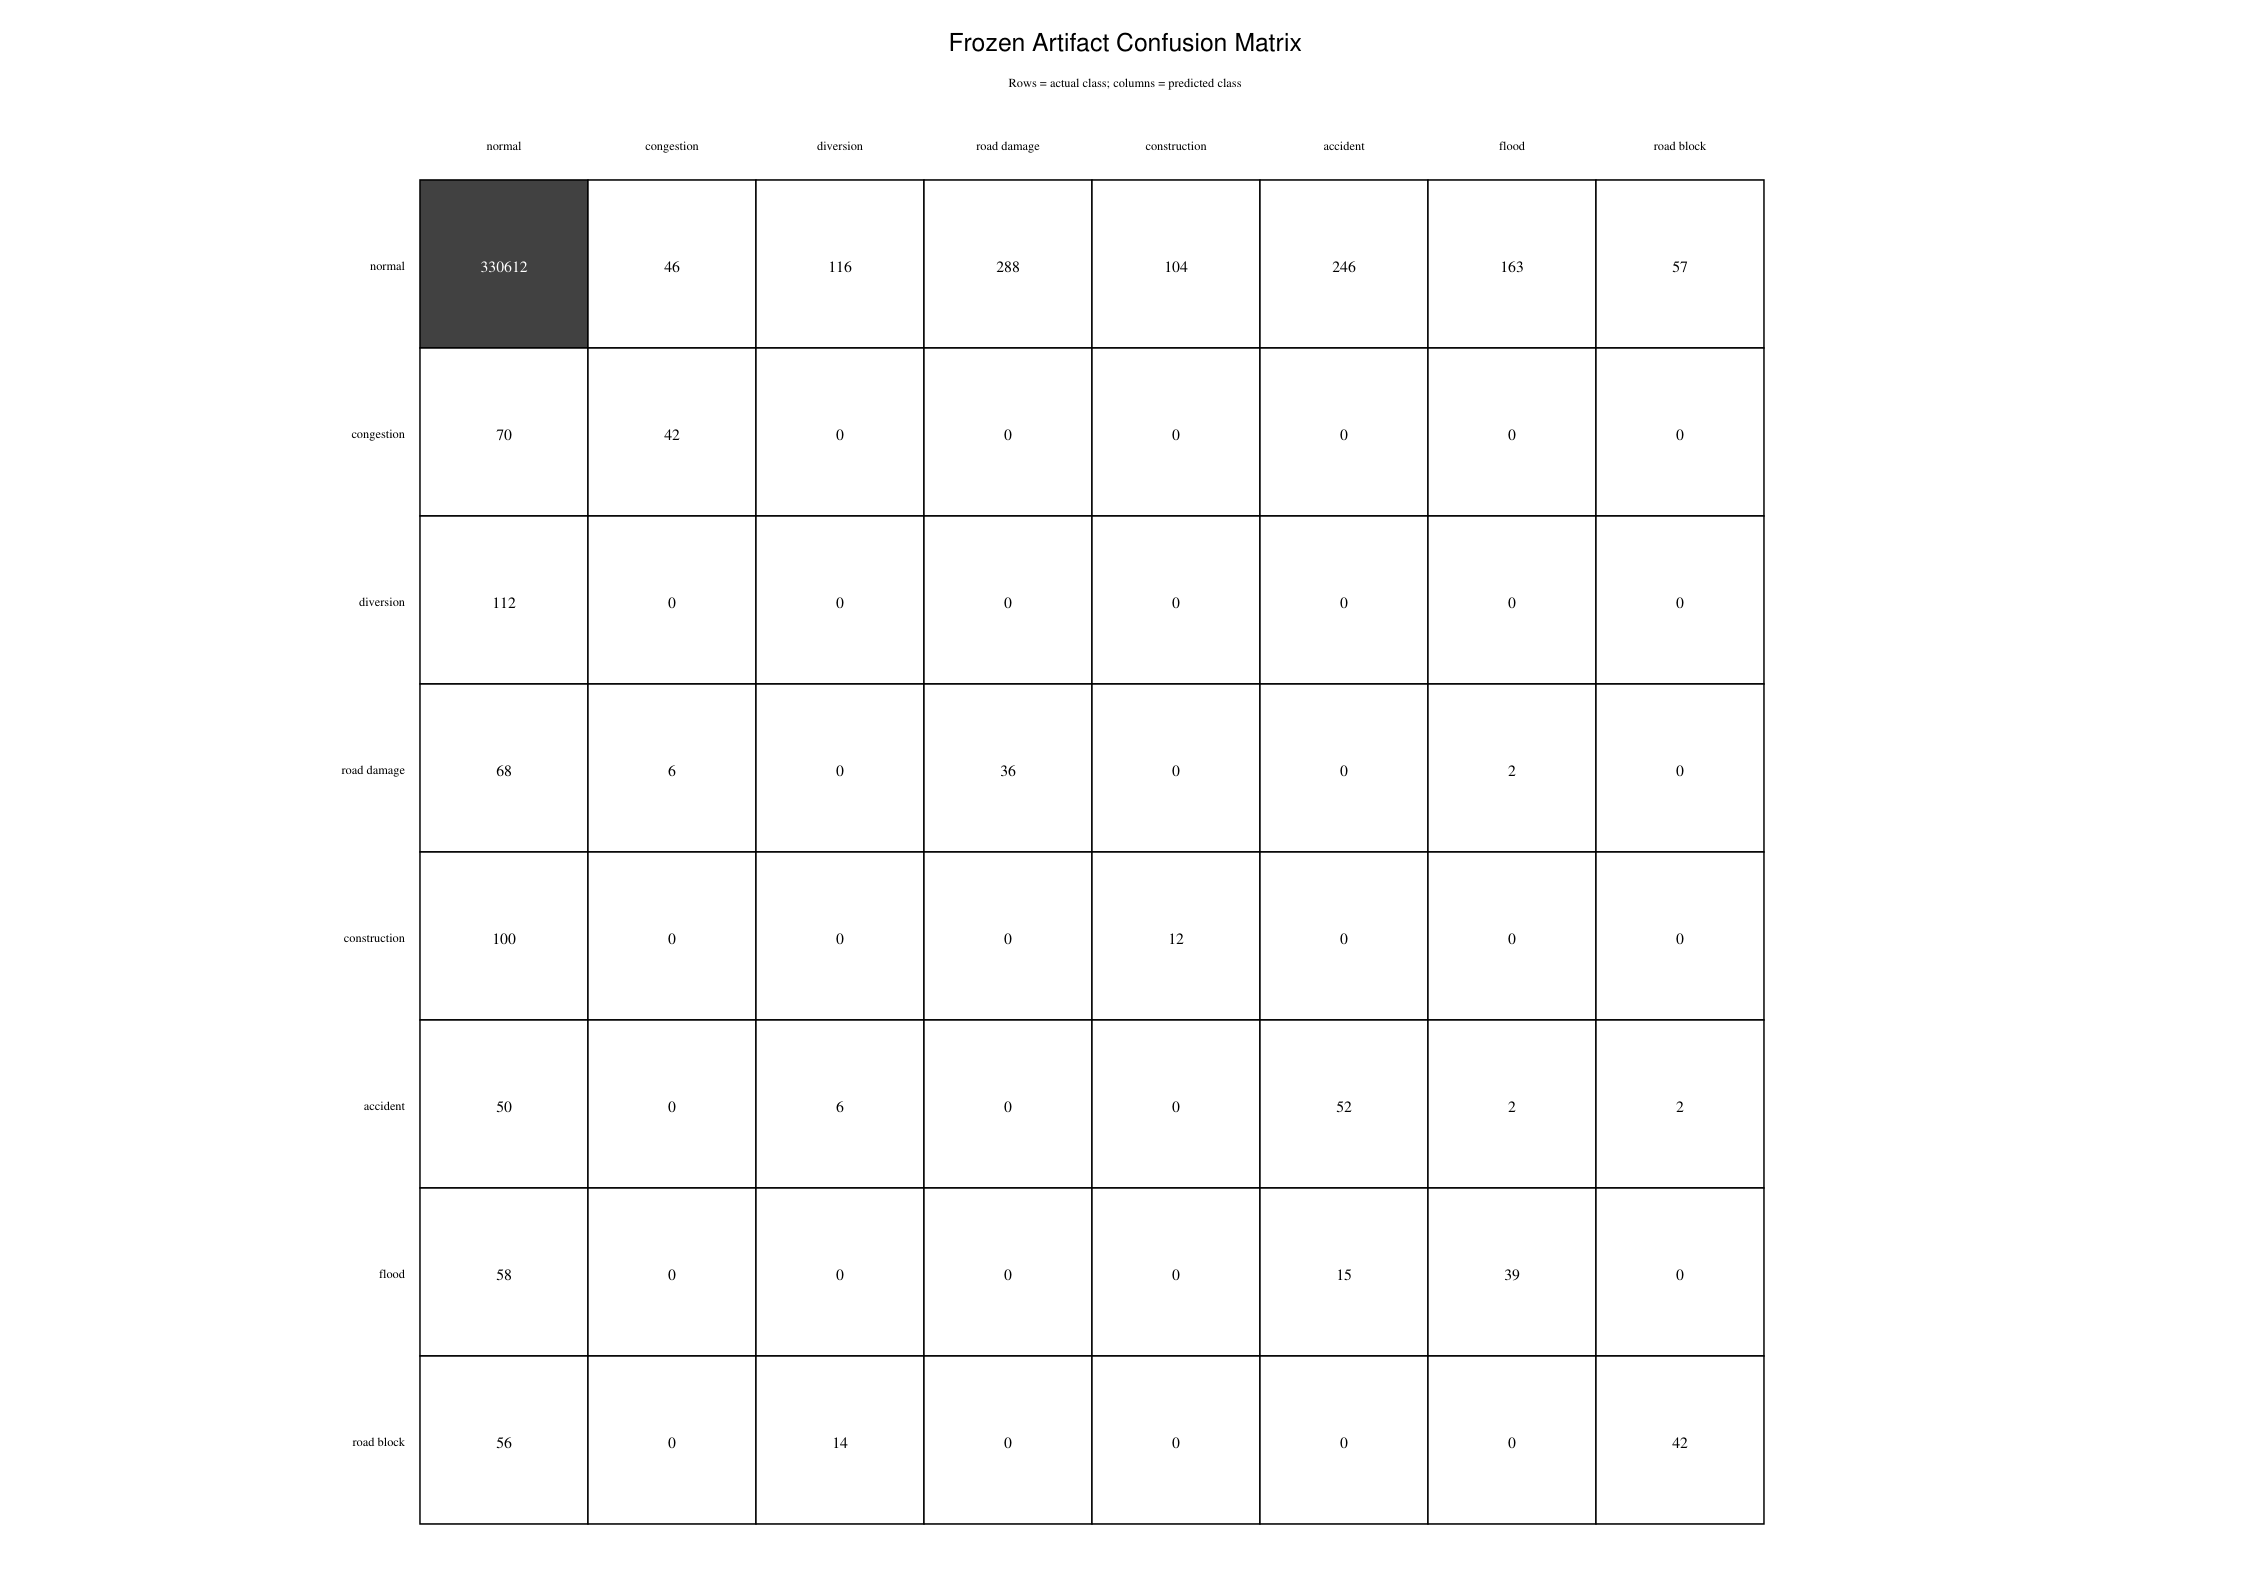
\includegraphics[width=0.9\textwidth,height=0.82\textheight,keepaspectratio]{fig_6_2.png}
\caption{Model Confusion Matrix}
\label{fig:6-2}
\end{figure}

The Backend and Frontend Test Evidence is illustrated in Figure~\ref{fig:6-3}.\par

\begin{figure}[p]
\centering
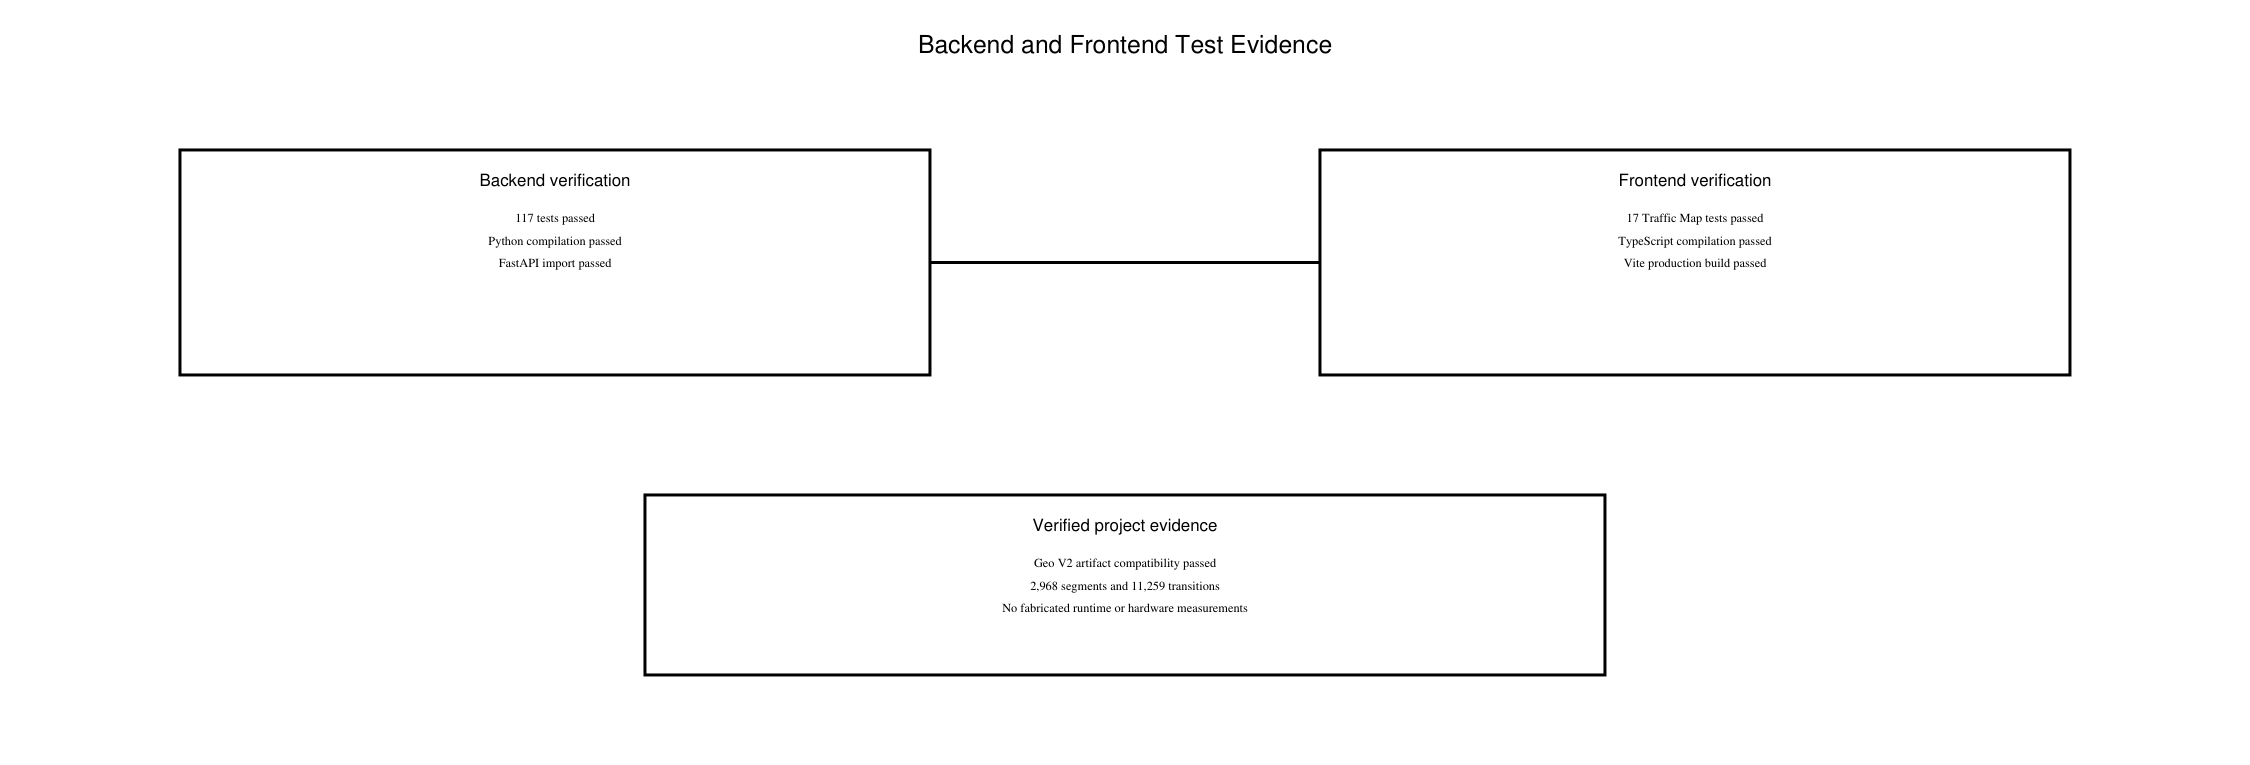
\includegraphics[width=0.9\textwidth,height=0.82\textheight,keepaspectratio]{fig_6_3.png}
\caption{Backend and Frontend Test Evidence}
\label{fig:6-3}
\end{figure}

\chapter{DEPLOYMENT, SECURITY AND PERFORMANCE}

\section{Deployment}

FedRouteAI is implemented as a modular application that can be deployed in a local development or demonstration environment. The main components include the frontend application, backend API services, database and spatial processing layer, machine learning model, and the federated learning~\cite{mcmahan2017,kairouz2021,beutel2020} components. The frontend provides the user interface through which traffic information, predictions, vehicle movement, road-network information, and routing results can be accessed. The backend provides the API layer connecting the frontend with the processing, machine learning, and database components. PostgreSQL~\cite{postgis} with PostGIS provides the spatial data layer required for storing and processing the road network and associated traffic information. The trained machine learning model is loaded by the backend inference component and used to generate traffic-event~\cite{han2019} predictions from the Geo V2 feature representation. The deployment architecture maintains separation between the major components so that they can be developed, tested, and operated independently. The basic application flow is:\par

\begin{center}\ttfamily\small Frontend  $\rightarrow$  Backend API  $\rightarrow$  Processing / ML Services  $\rightarrow$  PostgreSQL/PostGIS\end{center}

The federated learning process operates as a separate training workflow. The regional clients perform local training and contribute model updates to the aggregation process. The resulting global model can then be used by the runtime inference system. The current deployment is intended for an academic prototype~\cite{projsrc} and demonstration environment. It does not claim production-scale city-wide deployment or continuous large-scale~\cite{zhou2019,wang2020,khan2020} traffic-data processing.\par

The Local Deployment Architecture is illustrated in Figure~\ref{fig:7-1}.\par

\begin{figure}[p]
\centering
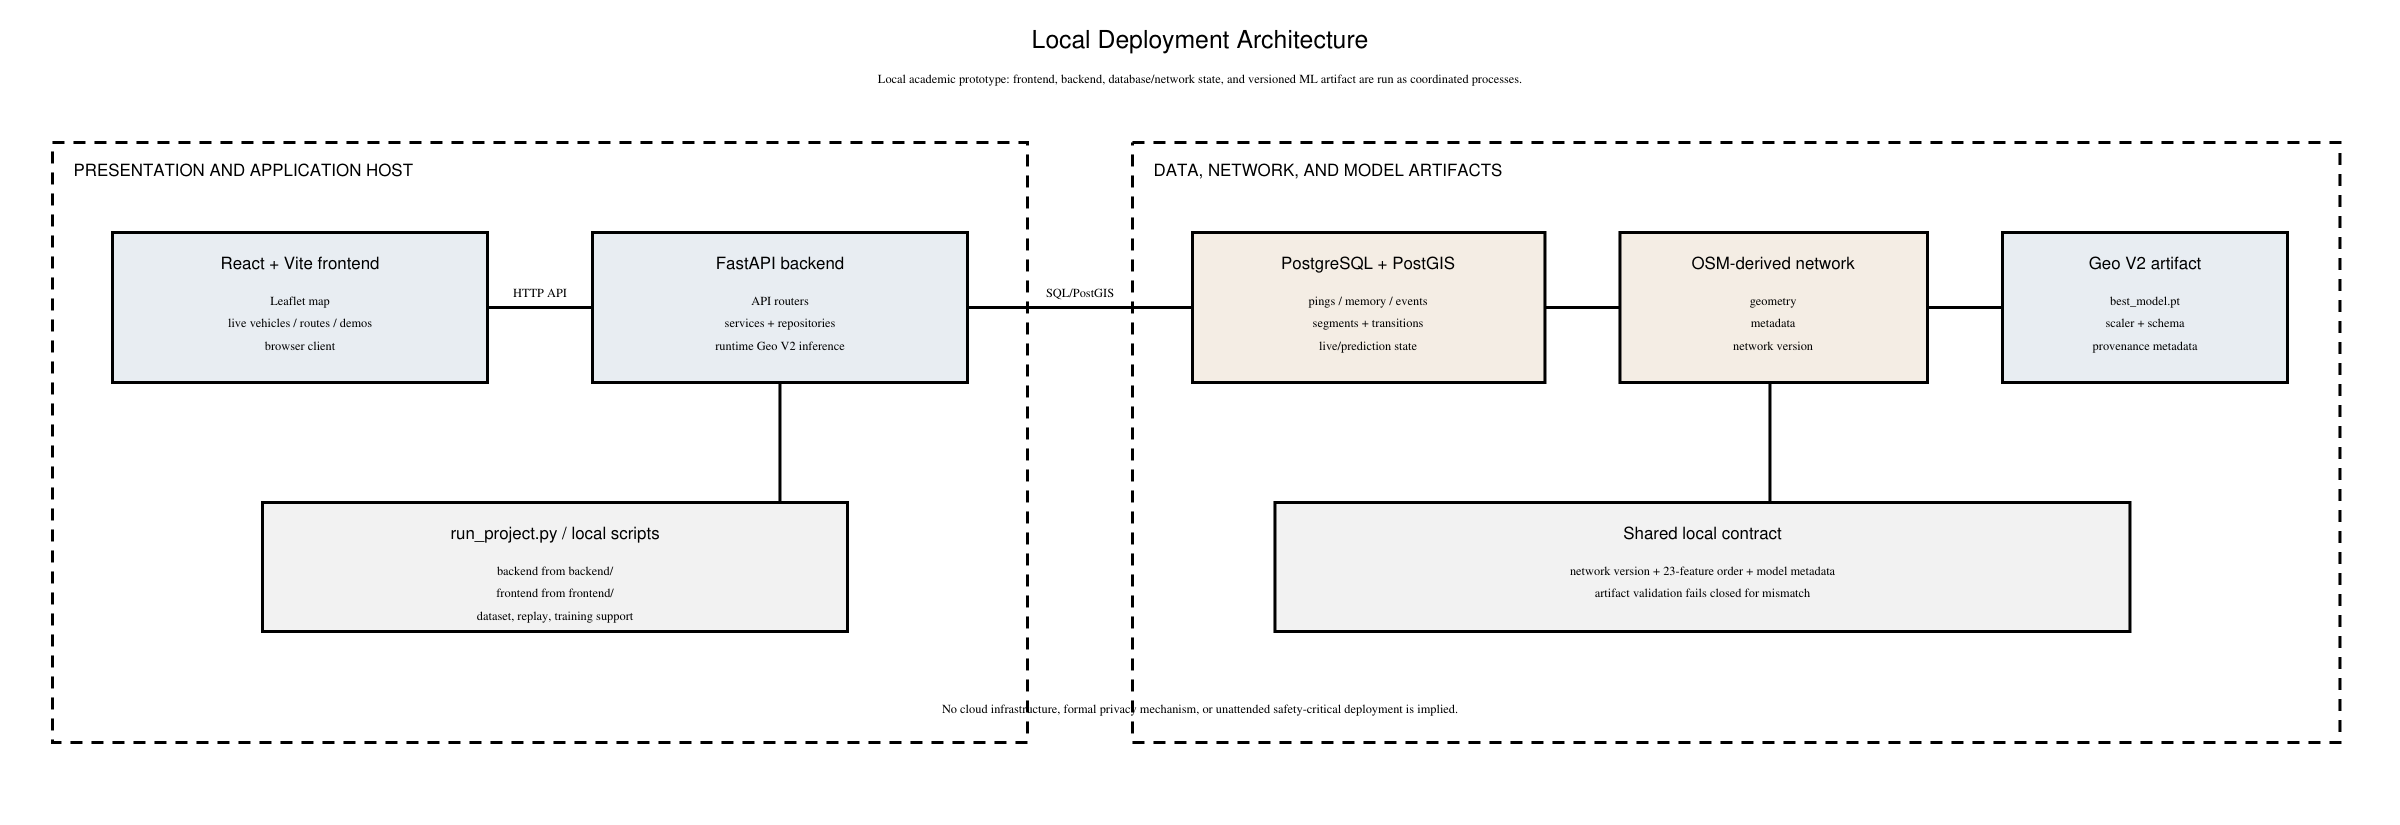
\includegraphics[width=0.9\textwidth,height=0.82\textheight,keepaspectratio]{fig_7_1.png}
\caption{Local Deployment Architecture}
\label{fig:7-1}
\end{figure}

\section{Security and Privacy}

Security is considered at the application and system-component level. The separation of the frontend, backend, database, and machine learning components helps establish clear interfaces between different parts of the application. The backend is responsible for validating and processing application requests before interacting with the underlying services and database. The model artifact~\cite{goodfellow2016,bishop2006,paszke2019} and feature-processing pipeline are also treated as controlled components of the application environment. Privacy~\cite{liu2020} is an important consideration because GPS and mobility data can potentially reveal information about vehicle movement patterns. The federated learning architecture reduces the requirement to transfer complete regional training datasets to a central location by allowing participating clients to perform local training. However, federated learning alone does not guarantee complete privacy. The current implementation does not include formal differential privacy~\cite{dwork2014,abadi2016,wei2020}, secure aggregation~\cite{kairouz2021,shokri2015}, or a formally defined privacy budget. Therefore, the privacy benefit provided by the current system should be described as reduced centralization of raw training data, rather than as a guarantee of privacy. Future versions of the system can strengthen privacy protection by incorporating formal privacy-preserving mechanisms such as differential privacy and secure aggregation.\par

\section{Performance}

Performance evaluation is used to determine whether the implemented system components operate within reasonable limits for the intended prototype environment. The machine learning model has an observed isolated inference time of approximately 0.414 ms per inference under the measured experimental conditions. This measurement represents warmed model inference and should not be interpreted as the response time or throughput of the complete FedRouteAI application. End-to-end application performance also depends on telemetry processing, road-segment association, Geo V2 feature construction, database access, API communication, and frontend rendering. These operations introduce additional processing overhead beyond the model inference stage. The reported performance therefore demonstrates the computational feasibility of the trained model within the prototype environment rather than production-scale system throughput. Performance results are also dependent on the hardware and software environment used during testing. For meaningful comparison or reproduction, the corresponding environment and configuration should be documented together with the measured results. The current implementation provides a suitable basis for future optimization involving distributed~\cite{wu2024} processing, asynchronous ingestion, caching, database optimization, and larger-scale deployment.\par

\section{Limitations}

The current deployment has several limitations that should be considered when interpreting the system results. The system is primarily evaluated as an academic prototype using geographically grounded synthetic traffic data. Consequently, the deployment does not demonstrate continuous operation over a large real-world traffic network. The current system also does not implement formal privacy mechanisms such as differential privacy or secure aggregation. Federated learning reduces the need to centralize raw regional training data, but additional mechanisms would be required for stronger privacy guarantees. The routing component uses a distance-based directed shortest-path approach. Traffic-event predictions are not currently incorporated into the route cost, so the system does not provide fully traffic-aware dynamic routing. The reported model-inference performance is an isolated measurement and does not represent complete application throughput. End-to-end performance would require evaluation under realistic traffic-data volumes and deployment conditions. These limitations define the current scope of FedRouteAI and provide a basis for future improvements in privacy, scalability, real-world validation, traffic-aware routing, and deployment.\par

\chapter{CONCLUSION AND FUTURE ENHANCEMENTS}

\section{Conclusion}

FedRouteAI presents an integrated traffic-intelligence prototype that combines federated learning~\cite{mcmahan2017,kairouz2021,beutel2020}, GPS-based traffic processing, spatial road-network information, machine learning, web visualization, and directed routing. The system processes GPS-derived vehicle telemetry by associating observations with road segments and aggregating them into segment-level traffic information. Historical traffic information is incorporated into the feature-construction process, and the resulting data are transformed into the defined 23-feature Geo V2 representation. The machine learning component uses an MLP~\cite{goodfellow2016,bishop2006,paszke2019}-based classifier to perform traffic-event~\cite{han2019} prediction. The federated learning architecture represents eight regional clients that perform local training and contribute model updates to the global aggregation process. Adaptive FedAvg~\cite{yuan2024,lu2024}~\cite{mcmahan2017} is used as part of the federated aggregation workflow. The spatial component uses OpenStreetMap~\cite{osm}-derived road-network information together with PostgreSQL~\cite{postgis}/PostGIS. This provides a consistent representation of road segments for traffic processing, prediction visualization, and routing. The backend provides APIs through which processed traffic information and model predictions can be accessed, while the React~\cite{react_leaflet}-based frontend provides an interactive map-based interface for viewing the road network, vehicle information, traffic conditions, predictions, and routes. The system also provides directed shortest-path routing using Dijkstra~\cite{dijkstra1959}'s algorithm. The current implementation uses distance-based routing, and traffic-event predictions are not currently used as dynamic route costs. Testing and validation were performed across the major system components, including backend services, frontend functionality, Geo V2 feature construction, model artifacts, routing, ingestion, build, and runtime behavior. The machine learning evaluation demonstrates the ability of the implemented MLP to perform traffic-event classification on the experimental dataset, while also showing the limitations associated with class imbalance~\cite{lu2024} and minority-event detection. Overall, FedRouteAI demonstrates the feasibility of integrating distributed~\cite{wu2024} learning, traffic-data processing, spatial information, machine learning prediction, visualization, and routing into a single reproducible academic prototype~\cite{projsrc}. The system establishes a foundation for further development while maintaining clear boundaries between training data, runtime observations, model predictions, and controlled demonstrations.\par

\section{Future Enhancements}

The current implementation provides several opportunities for future development. A major direction is the use of larger and continuously collected real-world traffic datasets. Real-world evaluation would allow the system to be tested under a wider range of traffic conditions and would provide a stronger basis for evaluating the generalization of the traffic-event classifier. The machine learning component can also be improved through better handling of class imbalance and additional experimentation with model architectures and training strategies. Improving the detection of minority traffic events is particularly important because the current experimental results show lower performance for some event categories. The federated learning architecture can be extended to support a larger number of geographically distributed clients. More realistic distributed deployments could also investigate communication~\cite{zhou2019,wang2020,khan2020} efficiency, asynchronous training, client variability, and more advanced aggregation strategies. Privacy~\cite{liu2020} protection can be strengthened by incorporating formal mechanisms such as differential privacy~\cite{dwork2014,abadi2016,wei2020} and secure aggregation~\cite{kairouz2021,shokri2015}. These mechanisms would provide additional protection beyond the reduction in raw-data centralization offered by the current federated learning approach. Another important enhancement is traffic-aware routing. The current routing system uses distance-based Dijkstra routing. Future versions could incorporate predicted traffic conditions, congestion levels, or traffic-event probabilities into route costs so that route selection can respond dynamically to traffic conditions. The system can also be extended toward larger-scale deployment through distributed telemetry ingestion, asynchronous processing, database optimization, caching, and cloud-based infrastructure. Such improvements would allow the architecture to be evaluated under more realistic traffic-data volumes. Further enhancements can also improve the visualization layer by providing richer traffic analytics, historical comparisons, event trends, and more detailed spatial information. These enhancements would help move FedRouteAI from an academic prototype toward a more comprehensive traffic-intelligence platform while preserving the modular architecture established in the current implementation.\par

\clearpage

\addcontentsline{toc}{chapter}{REFERENCES}

\begingroup
\setlength{\parindent}{0pt}
\renewcommand{\bibname}{REFERENCES}
\begin{thebibliography}{99}
\setlength{\itemsep}{2pt}
\bibitem{abadi2016} M. Abadi et al., "Deep Learning with Differential Privacy," Proceedings of ACM CCS, pp. 308-318, 2016.
\bibitem{beutel2020} D. J. Beutel et al., "Flower: A Friendly Federated Learning Research Framework," arXiv:2007.14390, 2020.
\bibitem{bishop2006} C. M. Bishop, Pattern Recognition and Machine Learning. Springer, 2006.
\bibitem{chen2016} C. Chen et al., "A Survey on Spatial-Temporal Data Mining for ITS," IEEE International Conference on Big Data, 2016.
\bibitem{dijkstra1959} E. W. Dijkstra, "A Note on Two Problems in Connexion with Graphs," Numerische Mathematik, vol. 1, pp. 269-271, 1959.
\bibitem{dwork2014} C. Dwork and A. Roth, "The Algorithmic Foundations of Differential Privacy," Foundations and Trends in Theoretical Computer Science, vol. 9, pp. 211-407, 2014.
\bibitem{elmanaa2022} I. El Manaa et al., "Road Traffic Anomaly Detection: A Survey," Digital Technologies and Applications, Springer, pp. 772-781, 2022.
\bibitem{gao2023} M. Gao et al., "Anomaly Traffic Detection in IoT Security Using Graph Neural Networks," Journal of Information Security and Applications, vol. 76, 2023.
\bibitem{goodfellow2016} I. Goodfellow, Y. Bengio, and A. Courville, Deep Learning. MIT Press, 2016.
\bibitem{han2019} X. Han, "Traffic Incident Detection: A Deep Learning Framework," IEEE Mobile Data Management, pp. 379-380, 2019.
\bibitem{hendrycks2017} D. Hendrycks and K. Gimpel, "A Baseline for Detecting Misclassified and Out-of-Distribution Examples in Neural Networks," ICLR, 2017.
\bibitem{kairouz2021} P. Kairouz et al., "Advances and Open Problems in Federated Learning," Foundations and Trends in Machine Learning, vol. 14, pp. 1-210, 2021.
\bibitem{khan2020} L. U. Khan et al., "Federated Learning for Edge Networks: Resource Optimization and Incentive Mechanism," IEEE Communications Magazine, vol. 58, pp. 88-93, 2020.
\bibitem{li2018} X. Li et al., "Deep Representation Learning for Trajectory Similarity Computation," IEEE ICDE, pp. 617-628, 2018.
\bibitem{liu2020} Y. Liu et al., "Privacy-Preserving Traffic Flow Prediction: A Federated Learning Approach," IEEE Internet of Things Journal, vol. 7, pp. 7751-7763, 2020.
\bibitem{lu2024} Z. Lu et al., "Federated Learning With Non-IID Data: A Survey," IEEE Internet of Things Journal, vol. 11, pp. 19188-19209, 2024.
\bibitem{mcmahan2017} H. B. McMahan et al., "Communication-Efficient Learning of Deep Networks from Decentralized Data," Proceedings of AISTATS, pp. 1273-1282, 2017.
\bibitem{paszke2019} A. Paszke et al., "PyTorch: An Imperative Style, High-Performance Deep Learning Library," NeurIPS, 2019.
\bibitem{raiyn2014} J. Raiyn and T. Toledo, "Real-Time Road Traffic Anomaly Detection," Journal of Transportation Technologies, vol. 4, pp. 256-266, 2014.
\bibitem{shokri2015} R. Shokri and V. Shmatikov, "Privacy-Preserving Deep Learning," Annual Allerton Conference, pp. 909-910, 2015.
\bibitem{su2019} H. Su et al., "A Survey of Trajectory Distance Measures and Performance Evaluation," VLDB Journal, vol. 29, pp. 3-32, 2019.
\bibitem{wang2020} X. Wang et al., "Convergence of Edge Computing and Deep Learning: A Comprehensive Survey," IEEE Communications Surveys and Tutorials, vol. 22, pp. 869-904, 2020.
\bibitem{wei2020} K. Wei et al., "Federated Learning With Differential Privacy: Algorithms and Performance Analysis," IEEE Transactions on Information Forensics and Security, vol. 15, pp. 3454-3469, 2020.
\bibitem{wu2024} J. Wu et al., "Topology-Aware Federated Learning in Edge Computing: A Comprehensive Survey," ACM Computing Surveys, vol. 56, pp. 1-41, 2024.
\bibitem{yang2022} G. Yang et al., "Anomaly Detection for Spatiotemporal Data in Action," ACM SIGKDD, pp. 4844-4845, 2022.
\bibitem{yuan2024} L. Yuan and D. Chen, "Adaptive Federated Learning with Non-IID Data," AHPCAI, SPIE, 2024.
\bibitem{zhang2025} R. Zhang et al., "A Survey on Federated Learning in Intelligent Transportation Systems," IEEE Transactions on Intelligent Vehicles, vol. 10, pp. 3043-3059, 2025.
\bibitem{zheng2015} Y. Zheng, "Trajectory Data Mining: An Overview," ACM Transactions on Intelligent Systems and Technology, vol. 6, pp. 1-41, 2015.
\bibitem{zhou2019} Z. Zhou et al., "Edge Intelligence: Paving the Last Mile of Artificial Intelligence With Edge Computing," Proceedings of the IEEE, vol. 107, pp. 1738-1762, 2019.
\bibitem{osm} OpenStreetMap Contributors, "OpenStreetMap," https://www.openstreetmap.org/, accessed 2026.
\bibitem{postgis} PostGIS Project Steering Committee, "PostGIS Documentation," https://postgis.net/documentation/, accessed 2026.
\bibitem{fastapi} FastAPI Documentation, https://fastapi.tiangolo.com/, accessed 2026.
\bibitem{react_leaflet} React and Leaflet Documentation, https://react.dev/ and https://leafletjs.com/, accessed 2026.
\bibitem{projsrc} FedRouteAI project technical sources: backend, frontend, tests, manifests, network loader, and frozen artifact metadata, accessed 2026.
\end{thebibliography}
\endgroup

\end{document}
